\RequirePackage[fleqn]{amsmath}
\RequirePackage{fix-cm}
%
%\documentclass{svjour3}                     % onecolumn (standard format)
%\documentclass[smallcondensed]{svjour3}     % onecolumn (ditto)
\documentclass[smallextended,natbib]{svjour3}       % onecolumn (second format)
%\documentclass[twocolumn]{svjour3}          % twocolumn
%
\smartqed  % flush right qed marks, e.g. at end of proof
%
\usepackage{graphicx}

%\usepackage{times}
%\usepackage{latexsym}
%\usepackage{multirow}
\usepackage{url}
\makeatletter
\makeatother
%\usepackage[hidelinks]{hyperref}
%\DeclareMathOperator*{\argmax}{arg\,max}

% \usepackage{times}
% \usepackage{url}
% \usepackage{latexsym}
% 
% \usepackage[fleqn]{amsmath}
% \usepackage{amssymb}
% \usepackage{amstext}
% \usepackage{amsthm}
% 
%\usepackage{cite}

\usepackage{amsfonts}
\usepackage{algorithm2e}
\usepackage{array}
\usepackage[caption=false,font=footnotesize]{subfig}
\usepackage{url}
\usepackage{tabularx}
\usepackage{numprint}
\usepackage{multirow}

\newcommand{\bs}{\boldsymbol}  
\newcommand{\wrtd}{\mathrm{d}}

\makeatletter
\makeatother %some sort of hack related to the symbol @

%%%%%%%%%%%%%%%%%%%%%%%%%%%%%%%%%%%%%%%%%%%%%%%%%%%%%%%%%%%%%%%%%

\title{ 
Scalable and Sparse: Bayesian Preference Learning with Crowds
}

\author{Edwin Simpson 
\and Iryna Gurevych \\
}
\institute{Ubiquitous Knowledge Processing Lab, Dept. of Computer Science, Technische Universit\"at Darmstadt, Germany\\
              \email{\{simpson,gurevych\}@ukp.informatik.tu-darmstadt.de}
}
\date{Received: date}
\begin{document}

% do not exceed 20 pages including references

\maketitle

\begin{abstract}
We show how to make collaborative preference learning work at scale and how it can be used to learn
a target preference function from crowdsourced data or other noisy preference labels. 
The collaborative model captures the reliability of each worker or data source and models their biases and error rates. 
It uses latent factors to share information between similar workers and a target preference function.
We devise an SVI inference schema to enable the model to scale to real-world datasets.
Experiments compare results using standard variational inference, laplace approximation and SVI.
On real-world data we show the benefit of the personalised model over a GP preference learning approach 
that treats all labels as coming from the same source,
as well as established alternative methods and classifier baselines.
We show that the model is able to identify a number of latent features for the workers and for textual arguments.
\end{abstract}

% For peer review papers, you can put extra information on the cover
% page as needed:
% \ifCLASSOPTIONpeerreview
% \begin{center} \bfseries EDICS Category: 3-BBND \end{center}
% \fi
%
% For peerreview papers, this IEEEtran command inserts a page break and
% creates the second title. It will be ignored for other modes.
%\IEEEpeerreviewmaketitle

%%%%%%%%%%%%%%%%%%%%%%%%%%%%%%%%%%%%%%%%%%%%%%%%%%%%%%%%%%%%%%%%%

\section{Introduction}\label{sec:intro}

Many tasks are more suited to pairwise comparisons than classification etc. 
Crowds of non-expert annotators may label more accurately if presented with pairs. 
Implicit feedback may be taken from user actions in an application that can be represented as a preference, such as choosing
an option over other options.

There are several works for learning from noisy pairwise comparisons so far (Horvitz et al. 2013 or something like that?). 
However, these do not provide a way to take account of item features or to model different but valid subjective viewpoints. 
They assume there is a single ground truth and can therefore model only one task and one user's (or a consensus of all users) preferences at once. 

Work by Felt et al. 2015, Simpson et al. 2015 etc. shows that item features are particularly useful when combining crowdsourced data. A Gaussian process has not been tested for this purpose before?

GP preference learning presents a way to learn from noisy preferences but assumes constant noise and a single underlying preference function. 
The collaborative Gaussian process (Houlsby et al. 2012) learns multiple users' preferences. 
However existing implementations do not scale and do not identify ground truth. 

We show how to scale it using SVI and how to use the model to identify ground truth from subjective preferences. 

%Things we assume are discussed in the intro:
% -- recommendation -- item-item similarity, user-user similarity (CF), user-item matching
% -- learning from implicit preferences/user actions
% -- need to handle sparsity i.e. most pairs of users/items not labelled
% -- noisiness of pairwise labels? (btw can we use our model to combine implicit labels for a single user --> ground truth for this user --> not all sources of data agree with true orderings). 
% -- benefits of BMF
% -- use of GPs for BMF?
% -- Older learning-to-rank algorithms: 
%Learning to rank from pairwise comparison data has been studied for document retrieval systems
% 2. R. Herbrich, T. Graepel, K. Obermayer, "Large margin rank boundaries for ordinal regression" in , MIT Press, 2000.
% Show Context

% a learning algorithm was developed by extending AdaBoost in [3]
% 3. Y. Freund, R. D. Iyer, R. E. Schapire, Y. Singer, "An efficient boosting algorithm for combining preferences", Journal of Machine Learning Research, vol. 4, pp. 933-969, 2003.
% Show Context

% A simple probabilistic model based on a neural network, called RankNet, was introduced in [4] 
% 4. C. J. C. Burges, T. Shaked, E. Renshaw, A. Lazier, M. Deeds, N. Hamilton, G. N. Hullender, "Learning to rank using gradient descent", ICML, pp. 89-96, 2005.
% T. Joachims, "Optimizing search engines using clickthrough data", KDD, 2002.

%an SVM algorithm was generalized in [6] to learn a linear function for ranking
% 6. T. Joachims, "Optimizing search engines using clickthrough data", KDD, 2002.


%uchida2017entity -- learning preferences from user reviews
%APRIL paper from Alex? As a motivating example of why we need to learn preference function.

% A crowd may not necessarily consist of individual human annotators working towards a common goal of annotating a dataset. 
% It may be separate users of a system, whose individiual preferences we wish to predict,
% or we may treat the same user carrying out different tasks as a separate individual.  
% Each user may also generate labels for different types of user interaction.
% Hence, we can go beyond simple user-item matrices to treat each type of annotation  
% as a different 'user', and thereby combine different sources of information.
% Like the workers in a crowd, each source of annotations has a particular correlation with a ground truth
% that we wish to predict, i.e. the preferences for a particular user in a specific context.
% We must learn this correlation by identifying the ground truth from either explicit user ratings
% or consensus between relevant sources of information, defined a priori.

In this paper, we develop methodology to solve the following questions:
\begin{enumerate}
  \item How can we learn a rating function over large sets of items given a large number of pairwise comparisons?
  \item How do we account for the different personal preferences of annotators when inferring the ground truth?
\end{enumerate}
To answer these questions we make the following technical contributions:
\begin{enumerate}
 \item We propose a method for predicting either gold-standard or personalized ratings by aggregating crowdsourced preference labels using a model of the noise and biases of individual annotators. % say why this is not possible with Dawid and Skene
  \item %To enable collaborative preference learning % collaborative preference learning needs to be defined above
   To enable this method to scale to large, real-world datasets, we develop
   stochastic variational inference for Bayesian matrix factorization and Gaussian process preference learning.
  \item To expedite hyper-parameter tuning, we introduce a technique for gradient-based length-scale optimization of Gaussian processes.
\end{enumerate}

The next section of the paper discusses related work.
We then we develop our model for preference learning from crowds in Section \ref{sec:model},
followed by our proposed inference method in Section \ref{sec:inf} and
hyper-parameter optimisation technique in Section \ref{sec:ls}.
Then, in Section \ref{sec:expts}, 
we evaluate our approach empirically, showing first its behaviour on synthetic data, 
then its scalability and predictive performance on several real-world datasets.

% Note that Khan's method does not need factorization assumptions in the approximate posterior.
% Instead, they have no prior over v (item features).
% They have a diagonal covariance for the user features -- cheap. 
% They need a separate GP per user but it seems like this is not a problem in practice -- I guess
% the method scales linearly with no. users. In our case, we model covariance between users, so
% scaling is poor unless you can use inducing points or diagonal covariance.


\section{Related Work}
\label{sec:rw}

\subsection{Pairwise Preference Learning} 

To obtain a ranking from pairwise labels, 
many preference learning methods model
the user's choices as a random function of the latent 
\emph{utility} of the items.
Inferring the utilities of items allows us to rank them, estimate numerical ratings
and predict pairwise labels.
Many popular instances of this approach, known as a \emph{random utility model}~\citep{thurstone1927law},
are variants of  
the Bradley-Terry (BT) model~\citep{bradley1952rank,plackett1975analysis,luce1959possible},
or the Thurstone-Mosteller model, also known as \emph{Thurstone case V}~\citep{thurstone1927law,mosteller2006remarks}.
Examples include best-worst scaling~\citet{marley2005some}, which extends the BT model,
and TrueSkill~\citep{herbrich2007trueskill}, a Thurstone case V model that learns 
the skill of game players by treating match outcomes as noisy pairwise labels.
Recent work on the BT model has analysed bounds on error rates~\citep{chen2015spectral}, 
sample complexity~\citep{shah2015estimation}
and developed computationally efficient active learning~\citet{li2018hybrid}.
However, these examples do not consider input features.
Another commonly-used ranking method, SVM-rank~\citep{joachims2002optimizing},
predicts pairwise labels from input features, but optimises
pairwise label prediction directly without a random utility model.
\emph{Gaussian process preference learning (GPPL)}
provides a Bayesian treatment of the random utility model,
using input features to predict the utilities of test items and share information
between similar items~\citep{chu2005preference}.
Here, we build on GPPL to provide a scalable approach that can 
model the preferences of crowds of users.

\subsection{Annotator Disagreements when Estimating a Consensus}

Much of the previous work on preference learning from crowdsourced data 
treats disagreements as annotation errors and infers only the consensus,
rather than modelling personal preferences.
For instance, 
\citet{chen2013pairwise} and \citet{wang2016blind} 
tackle annotator disagreement %between annotators in a crowd 
using Bayesian approaches that learn the labelling accuracy of each worker.
Recently, \citet{pan2018stagewise} and \citet{han2018robust} 
introduced scalable methods that extend this idea from pairwise labels
to noisy \textit{k}-ary preferences,
i.e., totally-ordered subsets of $k$ items.
\citet{fu2016robust} improved SVM-rank by identifying outliers in crowdsourced data
that correspond to probable errors,
while \citet{uchida2017entity} extend SVM-rank to account for different levels of confidence in each pairwise annotation expressed by the annotators.
%TODO decide if this should be added.
%For crowdsourced classification tasks, \citet{simpson2017bayesian} show that modelling 
%individual annotator noise levels in combination with a Gaussian process can improve performance, but this has not yet been adapted for preference learning.
However, while these approaches differentiate the level of \emph{noise}
for each annotator,
personal preferences also introduce labelling \emph{bias}, 
as the differences between users are not random but depend on the items considered.
With small numbers of labels, these biases may reduce the accuracy of the estimated
consensus.
Furthermore, previous aggregation methods for crowdsourced preferences
do not consider the item features,
so cannot predict the utility of test items with no or very few labels~\citep{chen2013pairwise,wang2016blind,han2018robust,pan2018stagewise,li2018hybrid}.
Our approach goes beyond these methods
by predicting personal preferences
and incorporating item features into the model.

\subsection{Inferring Personal Preferences for Members of a Crowd}

A number of methods use matrix factorisation to predict personal preferences 
for members of a crowd from pairwise labels,
including 
\citet{yi_inferring_2013}, who focus on small numbers of pairs per user,
and \citet{salimans2012collaborative}, who apply Bayesian matrix factorisation to 
better handle sparse data.
In matrix factorisation, each individual's preferences are represented 
by a mixture of latent functions.
\citet{kim2014latent} do not apply matrix factorisation, but instead
assume that pairwise labels depend on one of several latent rankings.
However, these techniques do not account for any input features for prediction.

%crowdranking \citet{yi_inferring_2013} uses the crowd to make up for the fact that a target user has small data -- it's a form of collaborative filtering with pairwise labels using a non-Bayesian inference algorithm.
% Several other works learn multiple rankings from crowdsourced pairwise labels
% rather than a single gold-standard ranking, 
% but do not consider the item or user features so cannot extrapolate to new users or 
% items~\citep{yi_inferring_2013,kim2014latent}. 
% Both \citet{yi_inferring_2013} and learn a small number of
% latent ranking functions that can be combined to construct personalized preferences, 
% although neither provide a Bayesian treatment to handle data sparsity.
%include the work on collaborative GPPL
%Several extensions of BMF use Gaussian process priors over latent factors 
%to model correlations between 
%items given side information or observed item features~\citep{adams2010incorporating,zhou2012kernelized,houlsby2012collaborative,bolgar2016bayesian}. 
%However, these techniques are not directly applicable to 
%learning from pairwise comparisons 
%as they assume that the observations are Gaussian-distributed numerical ratings~\citep{shi2017survey}. 

A number of other methods use Gaussian processes 
for personal preference prediction, 
such as by \citet{guo2010gaussian}, who propose a joint Gaussian process over the
space of users and features. Since this scales cubically
in the number of users, \citet{abbasnejad2013learning} 
propose to cluster the users into behavioural groups.
However, distinct clusters do not
allow for collaborative learning between users with partially overlapping preferences, e.g. two users may both like one genre of music, 
while having different preferences over other genres. 
\citet{khan2014scalable} instead learn a GP for each user,
then add a matrix factorization term that performs collaborative filtering.
However, this approach does not model the relationship between
 input features and the latent factors,
 unlike \citet{lawrence2009non} who place GP priors over latent item components.
 Neither of these last two methods
 give a fully Bayesian treatment to the model, as the the users' latent features
 are optimised rather than marginalised.
An alternative is \emph{Collaborative GP (collabGP)}~\citep{houlsby2012collaborative},
which uses a latent factor model, where each latent factor has a Gaussian process prior. 
This allows the model to take advantage of the input features of both
users and items when learning the latent factors. 
However, unlike the approach we propose here, 
none of the methods to date jointly model both consensus 
and personal preferences in a fully-Bayesian manner,
which is needed to handle small amounts of data for both users and items
and account for personal biases when inferring the consensus.
Furthermore, the existing GP-based approaches
suffer from scalability issues due to limitations of their inference methods.

 % PCA: Gaussian noise. "The classical PCA converts a set of samples with possibly correlated variables into another   
 % set of samples with linearly uncorrelated variables via an orthogonal transformation [1]. Based on this, PCA
 % is an effective technique widely used in performing dimensionality reduction and extracting features." -- Shi et al 2017. shi2017survey
 % SVD: like PCA with the mean vector set to zeroes.
 % variations of PCA: for handling outliers or large sparse errors
 % most matrix factorizations are special cases of PCA and in practice do not consider the mean vector.
 % probabilistic PCA: latent variables are unit isotropic Gaussians --> all have 0 covariance and 1 variance.
 % Bayesian PCA: places priors on all latent variables.
 % Probabilistic factor analysis: assumes different variances on each of the latent factors.
 % Probabilistic matrix factorisation: ignores the mean. --> I.e. can be done with SVD
 % I think this means our method is a form of PFA? But extended to consider correlations in the weights.
 % NMF: as matrix factorisation but the low-rank matrices are non-negative.


\subsection{Scalable Approximate Bayesian Inference}

%Scalability of BMF
Many of the approaches for modelling individual user preferences use matrix factorization 
to share information between users and items,
which benefits from a Bayesian treatment to reduce the effects of overfitting or noisy data~\citep{saha2015scalable}.
Recent work on scalable Bayesian matrix factorization focuses on distributing and 
parallelising inference but %these approaches do not make use of input features and 
are not directly applicable when Gaussian processes are used to integrate input features
 ~\citep{ahn2015large,saha2015scalable,vander2017distributed,chen2018large}. 
%This paper focuses instead on reducing computational and memory costs, 
%although the method we propose is amenable to parallelization.

%Scalability of GPs
Models that combine Gaussian processes with non-Gaussian likelihoods 
require approximate inference methods that often scale poorly with 
the amount of training data available. 
Established methods such as the Laplace approximation 
and expectation propagation~\citep{rasmussen_gaussian_2006} have
computational complexity $\mathcal{O}(N^3)$ with $N$ data points
 and memory complexity $\mathcal{O}(N^2)$. 
For collaborative GPPL, \citet{houlsby2012collaborative}
propose a  kernel for pairwise 
preference learning and use a sparse
\emph{generalized fully independent training conditional} (GFITC) 
approximation~\citep{snelson2006sparse} to reduce the computational complexity to $\mathcal{O}(PM^2 + UM^2)$ and 
memory complexity to $\mathcal{O}(PM + UM)$,
where $P$ is the number of pairwise labels, 
$M \ll P$ is a fixed number of inducing points, 
and $U$ is the number of users.
However, this is not sufficiently scalable
for very large numbers of users or pairs, 
due to increasing memory consumption 
and optimisation steps that cannot be run in parallel on subsets of the data, 
since the objective function is a not a sum over data points.
%The marginal likelihood does not factor between data points -- updating for one data point may not 
% improve the marginal likelihood. If the objective function is a sum of terms, we can do gradient 
% descent steps on each term independently.  
%Updates  to the individual factors are not gradient descent steps for the overall objective 
%-- local objective only.
% This means they have some sequential dependencies on one another, so I don't know what
% happens if you do them out of order.
The GP over pairs also means that it does not output posteriors for 
the utilities of individual items, which are useful for ranking,
and can only be trained using pairwise labels, even if observations of the utilities
are available.

To handle large numbers of pairwise labels, \citet{khan2014scalable}
develop a variational EM algorithm and sub-sample pairwise data rather than learning from the complete training set.
An alternative is \emph{stochastic variational inference (SVI)}~\citep{hoffman2013stochastic}, 
which updates an approximation to the posterior using 
a different random sample of the training data at each iteration. 
This allows the approximation to make use of all training data over a number of 
iterations, while limiting training costs per iteration.
SVI has been successfully applied to Gaussian process regression~\citep{hensman2013gaussian} and classification~\citep{hensman2015scalable},
further improving scalability over existing sparse approximations.
For multi-output GPs, ~\citet{nguyen2014collaborative} introduce an SVI approach where 
each output is a weighted combination of shared latent functions plus a latent function specific to that output. 
They apply their method to capture dependencies between regression tasks,
treating the weights for the shared latent functions as hyperparameters. 
In this paper, we also use shared latent functions to capture dependencies between different users' preferences,
but introduce a Bayesian treatment of the weights using a GP over latent user features,
and integrate a non-Gaussian likelihood into the SVI framework to enable learning from pairwise labels.
An SVI method for preference learning that places a GP over items, rather than pairs, 
was previously applied by ~\citet{simpson2018finding}.
However, this method, a variant of GPPL,
did not consider the different preferences of individual users.
Here, we propose a new SVI method, crowdGPPL, aimed at a different task: 
jointly modelling personal preferences of users and the crowd consensus
using a combination of Gaussian processes and Bayesian matrix factorisation.
In Section \ref{sec:inf},
we provide the full details of the SVI method for 
both GPPL, as these were not previously published, then extend the scheme to crowdGPPL.

\todo{ add in table of notations (maybe in the appendix)}

\section{Bayesian Preference Learning for Crowds}\label{sec:model}

%%%% Notes

% Title or name of the model: 
% -- cannot decide this until we get most of the paper complete: will emphasis be on crowds? distilling ground truth
% from noisy sources (Bayesian preference learning for fusing unreliable sources)? user preferences/collaborative filtering?
% -- need a new name to differentiate from Houlsby et al. and Khan et al.?
% -- what are the differences in the model? Let's get the model written up.
% -- should also be some buzzword or word to generate interest: 
%    -- 'variational' is on the up, could be used in paper title
%    -- 'stochastic variational' is also on the up
%    -- 'crowdsourcing' on the way down as at 2010 level
%    -- 'gaussian process' on the way up
%    -- 'matrix factorization' kind of on the way up
%    -- 'scalable' on the way up
%    -- 'interactive learning' on the way down
%    -- 'preference learning' flattish, may be on way up slowly
% -- aimed at crowdsourcing problems (uses a common mean function as consensus?)
% -- other parameters for importance of features?
% -- combined preference learning? Preference aggregation? Collaborative crowdsourced preference learning? Bayesian preference learning for crowds? another word for 'multi-user' or 'many users and many items' vs. crowds?

% TO ADD: Why does the variance in f cancel out when predicting the probability of a pairwise label?
% TO ADD: Why does \sigma disappear if we learn the output scale.

% We also estimate the output scale of the GPs, the latent components, and item bias as part of the 
% variational approximation allowing us to estimate these parameters in a Bayesian manner without 
% resorting to maximum likelihood approaches.

% mention how the noise model deals with inconsistencies in preferences

% \begin{enumerate}
% \item What are the benefits of Bayesian methods and Gaussian processes in particular?
% \item The proposal by \citep{chu2005preference} shows how the advantages of a Bayesian
% approach can be exploited for preference learning by modifying the observation model

% Extensions:
% -- how do we replace the GP with a NN?
% -- would this move us from a Bayesian to an ML solution?
% -- maybe save this for future work? Or add a few lines if we can make it fit with the theme of the paper.
% -- another is to replace the fixed number of clusters with a CRP, then the whole thing can be nonparameteric preference learning with crowds.

%\subsection{Modeling Pairwise Preferences}

% Include the case for one user -- preferences may depend on a number of observed features.

%TODO items or instances?
%TODO prefer the use of 'utility' to 'value' since there is some uncertainty (the evaluations by the users can flip at random)

% this should be introduced in section 1. \citep{handleycomparative} -- compares BT with TM models
For a pair of items, $a$ and $b$, 
$a \succ b$ indicates that $a$ is preferred to $b$.  
% %\begin{equation}
% $y(a, b) = \begin{cases}
% 1 & a \succ b \\
% 0 & b \succ a
% \end{cases}$.
% %\end{equation} 
We assume that items have latent \emph{utilities},
$f(\bs x_a)$ and $f(\bs x_b)$, that represent their value to a user,
and that the 
utility $f(\bs x_a) : \mathbb{R}^D \mapsto \mathbb{R}$ 
is a function of the item's features, where $\bs x_a$ is a vector of length $D$
containing the features of item $a$.
Hence if $f(\bs x_a) > f(\bs x_b)$, then $a \succ b$.
We record the outcome of a comparison between $a$ and $b$ as 
a pairwise label, $y(a, b)$.
Assuming that pairwise labels never contain errors,
then $y(a, b)=1$ if $a \succ b$ and $0$ otherwise.

\citet{thurstone1927law} proposed the \emph{random utility model},
which relaxes the assumption that pairwise labels, $y(a, b)$,
are always consistent with the ordering of $f(\bs x_a)$ and $f(\bs x_b)$.
Under the random utility model, the likelihood $p(y(a,b)=1)$ 
increases as $f_a - f_b$ increases, i.e.,
as the utility of item $a$ increases
relative to the utility of item $b$.
However, since $0 < p(y(a,b)=1) < 1$, the model 
is uncertain about the value of $y(a,b)$,
which accommodates labelling errors or
inconsistency in a user's choices at different points in time.
The uncertainty is lower if the values $f_a$ and $f_b$ are further apart, 
which reflects greater consistency in a user's choices
when their preferences are stronger.
 
The random utility model is defined by a likelihood function that
maps the utilities to $p(y(a,b))$.
Two important random utility models for pairwise labels are the Bradley-Terry model ~\citep{bradley1952rank,plackett1975analysis,luce1959possible},
which assumes a logistic likelihood,
and the Thurstone-Mosteller model, also known as \emph{Thurstone case V}~\citep{thurstone1927law,mosteller2006remarks}, which assumes a probit likelihood.
%or the Thurstone-Mosteller model.
%\begin{align}
%p(y(a, b) | f) & = \frac{1}{1 + \exp( f(\bs x_a) - f(\bs x_b) ) }
%\end{align}
In the Thurstone case V model, 
noise in the observations is explained by a Gaussian-distributed noise term, $\delta \sim \mathcal{N}(0, \sigma^2)$:
\begin{align}
 p(y(a, b) | f(\bs x_a) + \delta_{a}, f(\bs x_b) + \delta_{b} )  
 \hspace{0.9cm} & = \begin{cases}
 1 & \text{if }f(\bs x_a) + \delta_{a} \geq f(b) + \delta_{b} \\
 0 & \text{otherwise,}
 \end{cases} &
 \label{eq:thurstone}
\end{align}
Integrating out the unknown values of $\delta_a$ and $\delta_b$ gives:
\begin{align}
& p( y(a, b) | f(\bs x_a), f(\bs x_b) )  \nonumber\\
& = \int\!\!\!\! \int p( y(a, b) | f(\bs x_a) + \delta_{a}, f(\bs x_b) + \delta_{b} ) \mathcal{N}(\delta_{a}; 0, \sigma^2)\mathcal{N}(\delta_{b}; 0, \sigma^2) d\delta_{a} d\delta_{b} \nonumber\\
& = \Phi\left(\frac{f(\bs x_a) - f(\bs x_b)}{\sqrt{2\sigma^2}}\right) = \Phi\left( z \right), 
\label{eq:plphi}
\end{align}
where $z = \frac{f(\bs x_a) - f(\bs x_b)}{\sqrt{2\sigma^2}}$,
and $\Phi$ is the cumulative distribution function of the standard normal distribution,
meaning that $\Phi(z)$ is a probit likelihood. 

In practice, $f(\bs x_a)$ and $f(\bs x_b)$ must be inferred from
pairwise training labels, $\bs y$,
so that we obtain a posterior distribution over their values.
If we assume that this posterior is a multivariate Gaussian distribution,
then the probit likelihood allows us to analytically marginalise 
$f(\bs x_a)$ and $f(\bs x_b)$
to obtain the probability of a pairwise label:
\begin{align}
p(y(a,b)| \bs y) 
= \Phi(\hat{z}),& & \hat{z} = \frac{\hat{f}_a - \hat{f}_b}{\sqrt{2\sigma^2 + C_{a,a} + C_{b,b} 
- 2C_{a,b}} }, \label{eq:predict_z}
\end{align}
where $\hat{f}_a$ and $\hat{f}_b$ are the means and
$\bs C$ is the covariance matrix of the multivariate Gaussian over
$f(\bs x_a)$ and $f(\bs x_b)$.
This likelihood model is the basis of Gaussian process preference learning (GPPL)~\citep{chu2005preference}. 
Due to this mathematical convenience,
we also assume this pairwise label likelihood for the crowd
preference learning model proposed in this paper.
Here, in contrast to \citet{chu2005preference},
we simplify the formulation by assuming that $\sigma^2 = 0.5$,
which leads to $z$ having a denominator of $\sqrt{2 \times 0.5}=1$.
Instead, we model varying degrees of noise in the pairwise labels
by scaling $f$ itself, as we describe in the next section.
%Obtaining the posterior over $f$ is itself challenging, however, 
%and therefore in Section $\ref{sec:inf}$ we propose 
%an approximate inference method to address this problem.


\subsection{Single User Preference Learning}
%TODO check use of 'user' versus 'annotator' terminology throughout, especially in the intro. Is it explicit that the term 'user' is abstract and refers to any of these things?
We can model the preferences of a single user by assuming
a Gaussian process prior over the user's utility function, 
%is a function of item features and 
$f \sim \mathcal{GP}(0, k_{\theta}/s)$, where $k_{\theta}$ is a kernel function with hyperparameters $\theta$
and $s$ is an inverse scale parameter.
The kernel function takes numerical item features as inputs and determines the covariance between values of $f$ for different items. 
The choice of kernel function and its hyperparameters controls the shape and smoothness of the function 
across the feature space and is often treated as a model selection problem.
Typical kernel functions include the \emph{squared exponential} 
and the \emph{Mat\'ern}~\citep{rasmussen_gaussian_2006},
which both make minimal assumptions and are effective in a wide range of tasks. 
These functions assign higher covariance to items with similar feature values.
We use the kernel function $k_{\theta}$ to compute a covariance matrix $K_{\theta}$,
between a set of $N$ observed items with features $\{ \bs x_1, ..., \bs x_N \}$.

The model extends the original definition of
\emph{Gaussian process preference learning (GPPL)}~\citep{chu2005preference},
by introducing the inverse scale, $s$. 
We also assume that $s$ is drawn from a gamma prior, 
$s \sim \mathcal{G}(\alpha_0, \beta_0)$, with shape $\alpha_0$ and scale $\beta_0$.
The value of $1/s$ determines the variance of $f$,
and therefore 
the magnitude of differences between $f(\bs x_a)$ and $f(\bs x_b)$ for
items $a$ and $b$. This in turn affects the level of certainty
in the pairwise label likelihood as per Equation \ref{eq:plphi}.

Given a set of $P$ pairwise labels, %for a single user, 
$\bs y=\{y_1,...,y_P\}$,
where %the $p$th label, 
$y_p=y(a_p, b_p)$ is the preference label for items $a_p$ and $b_p$, % refers to items $\{ a_p, b_p \}$.
we can write the joint distribution over all variables as follows:
\begin{flalign}
p\left( \bs{y}, \bs f, s | k_{\theta}, \alpha_0, \beta_0 \right) 
=  \prod_{p=1}^P p( y_p | \bs f ) 
\mathcal{N}(\bs f; \bs 0, \bs K_{\theta}/s) \mathcal{G}(s; \alpha_0, \beta_0) %\nonumber \\
%=  \prod_{p=1}^P \Phi\left( z_p \right) 
%\mathcal{N}(\bs f; \bs 0, \bs K_{\theta}/s) \mathcal{G}(s; \alpha_0, \beta_0), &
\label{eq:joint_single}
\end{flalign}
where 
$\bs f = \{f(\bs {x}_1),...,f(\bs {x}_N)\}$
is a vector containing the utilities of the $N$ items referred to by $\bs y$,
and $p( y_p | \bs f ) = \Phi\left( z_p \right)$ is the pairwise likelihood (Equation \ref{eq:plphi}). 
We henceforth refer to this model simply as \emph{GPPL}.

\subsection{Crowd Preference Learning} \label{sec:crowd_model}

% 0. Consider multiple users, each with a set of observed features.
% 1. imagine augmenting the observed features with a number of latent features (this is kind of what Khan et al. do)
% 2. imagine that the latent features relate preference function values between items and users using the smallest number of features
% 3. hence the observed features are not needed given the latent features, but we can create a hierarchical model where the latent features depend on the observed ones if available.

To predict the individual preferences of users in a crowd,
we could assume an independent GPPL model for each user.
However, by modelling all users' preferences jointly, we can
exploit the correlations between different users' interests
to improve predictions when preference data is sparse,
and reduce the cost of storing separate models for all users.
Groups of users may share common interests over certain subsets of items,
for example, in a book recommendation task,
some users may share an interest in one particular genre 
but otherwise prefer different categories of books.
Identifying such correlations between users' interests helps to predict 
the preferences of users for whom we have only observed a small number of preferences.
This is the core idea of recommendation techniques such as collaborative filtering~\citep{resnick1997recommender} and matrix factorisation~\citep{koren2009matrix}.

As well as predicting individual preferences, 
we wish to predict the consensus by aggregating
preference labels from multiple users. 
If we do not account for the individual biases of different users
when predicting the consensus,
these biases may affect the consensus predictions,
particularly when data for certain items is only available from a small subset of users.
We address this problem by proposing \emph{crowdGPPL}, which jointly models 
the preferences of individual users as well as the underlying consensus of the crowd.
Unlike previous methods for inferring the consensus, 
such as \emph{CrowdBT}~\citep{chen2013pairwise}, we do not treat differences between individuals as simply the result of labelling errors, 
but instead assume that differences result from the users' subjective biases
towards particular items. 
 
% is there a better word than 'label sources' for the different sources of implicit feedback or other types of labeling?
%In a scenario with multiple users or label sources, 
For crowdGPPL, 
we represent utilities in a matrix, $\bs{F} \in \mathbb{R}^{N \times U}$,
with $N$ rows corresponding to items and $U$ columns corresponding to users. %, and entries are preference values.
We assume that $\bs F$ is the product of two low-dimensional matrices
plus a vector of consensus utilities, $\bs{t}$, of the $N$ items, as follows:
\begin{equation}
\bs{F} = \bs{V}^T \bs{W} + \bs{t},
\end{equation}
where $\bs{W} \in \mathbb{R}^{C \times U}$ is a latent representation
of the users,
$\bs{V} \in \mathbb{R}^{C \times N}$ is a latent representation of the items,
and $C$ is the number of latent \emph{components}, i.e., the dimension
of the latent representations.
The column $\bs v_{.,a}$ of $\bs V$, and the column $\bs w_{.,j}$ of $\bs W$,
 are latent vector representations of item $a$ and user $j$,
 respectively.
%Users with similar values for a certain feature will have similar preferences for 
%the subset of items with corresponding feature values. 
Each latent component corresponds to a utility function 
for certain items, which is shared by a subset of users.
For example, in the case of book recommendation,
one component could represent the membership of certain books to a particular
genre and the interests of certain users in that genre.
%Besides latent features, we may also observe a number of item features, $\bs x$,
%and . 
%There are two ways that observed features can be incorporated into the 
%model: (1) as additional dimensions of V or W (each feature cannot be a member of %both); (2) as input features on which V and W depend. The advantage of the latter is that 
%In the single user model, we assumed a single latent utility function, $f$, of the observed item features. 

For crowdGPPL, we assume that each row of $\bs V$, $\bs v_c=\{ 
v_c(\bs{x}_1),...,v_c(\bs{x}_N)\}$,  
contains evaluations of a latent function, 
$v_c\sim \mathcal{GP}(\bs 0, k_{\theta} /s^{(v)}_c)$,
of item features, $\bs x_a$,
where $k$ is a kernel function, $s^{(v)}_c$ is an inverse function scale,
and $\theta$ are kernel hyperparameters.
%Since our goal is to infer a consensus from a crowd as well as to model individual 
%users' preferences, 
We also assume that $\bs t = \{t(\bs {x}_1),...,t(\bs {x}_N)\}$
contains evaluations of a consensus utility function over item features,
$t\sim \mathcal{GP}(\bs 0, k_{\theta} /s^{(t)})$, which is shared across all users.
Similarly, each row $\bs w_c=\{w_c(\bs u_1),...,w_c(\bs u_U)\}$ 
of $\bs W$ contains evaluations of a latent function,
$w_c \sim \mathcal{GP}(\bs 0, k_{\eta} / s^{(w)}_c)$,
of user features, $\bs u_j$, 
with inverse scale $s^{(w)}_c$ 
and kernel hyperparameters $\eta$.
Therefore, the utilities in $\bs F$ are evaluations of a joint
preference function, $f$, which is a weighted sum over the latent functions:
\begin{flalign}
  f(\bs x_a, \bs u_j) = \sum_{c=1}^C  v_c(\bs x_a) w_c(\bs u_j) + t(\bs x_a),
\end{flalign}
where $\bs u_j$ are the features of user $j$ and $\bs x_a$ are the features of item $a$.
This model therefore assumes that items have an underlying consensus utility,
given by $t(\bs x_a)$,
and that individual user preferences then deviate from the consensus according
to $\sum_{c=1}^C  v_c(\bs x_a) w_c(\bs u_j)$. 
Hence, when inferring the consensus utilities, we can subtract the effect of individual
biases. The consensus can also help 
when inferring personal preferences for user-item combinations that are
not similar to the combinations in the training data, by
taking into account any objective quality or widespread appeal that an item may have.
%We provide a Bayesian treatment to matrix factorization by placing Gaussian process priors over the latent functions.
%differently for each user and item. For example, the observed user feature 'age' may correlate with some latent interests of users, but certain users will deviate from their peer group. 
% what happens if two users have identical features (say, the feature representation
% has only simple values, such as age in years)? They have 1-1 covariance, but there 
% is variance in the GP at one location, so both can be drawn separately from the prior.
%It is not necessary to learn a separate scale for $w_c$, since $v_c$ and $w_c$ are multiplied with each other, making a single $s^{(v)}_c$ equivalent to the product of two separate scales. 
%The choice of $C$ can be treated as a hyperparameter, or modeled using a non-parametric prior, such as 
%the Indian Buffet Process, which assumes an infinite number of latent components ~\citep{ding2010nonparametric}.
%This section described a Bayesian matrix factorization model, 
%which we will subsequently extend to a preference learning model for crowds of users and label sources. 
% joint distribution
% notes about problems with inference.
\todo{Page 7, equation (5): you might want to cite precedence to this form of equation
e.g. K. Mo, E. Zhong, and Q. Yang. Cross-task crowdsourcing. In Proceedings of the 19th ACM SIGKDD International Conference on Knowledge Discovery and Data Mining, KDD '13, pages 677-685, New York, NY, USA, 2013. ACM. ISBN 978-1-4503-2174-7. doi: 10.1145/2487575.2487593. URL http://doi.acm.org/10.1145/2487575.2487593.}

We combine the matrix factorization method with the preference likelihood of Equation \ref{eq:plphi}
to obtain a joint preference model for multiple users, \emph{crowdGPPL}:
%represent a consensus between users,
%if present, while allowing individual users' preferences to deviate from this value through $\bs V^T \bs W$. 
%Hence, $\bs t$ can model the underlying ground truth or consensus in crowdsourcing scenarios, or when using
%multiple label sources to learn preferences for one individual.
\begin{flalign}
p\left( \bs{y}, \bs V, \bs W, \bs t, s_1, ..., s^{(v)}_c, s^{(t)} | k_{\theta}, k_{\eta}, \alpha_0, \beta_0 \right) 
= \prod_{p=1}^P \Phi\left( z_p \right) 
\mathcal{N}(\bs t; \bs 0, \bs K_{\theta} /s^{(t)})
 && \nonumber \\ 
\mathcal{G}({s^{(t)}}; \alpha_0, \beta_0)\prod_{c=1}^C \left\{
\mathcal{N}(\bs v_c; \bs 0, \bs K_{\theta} /s^{(v)}_c) 
\mathcal{N}(\bs w_c; \bs 0, \bs L_{\eta}/s^{(w)}_c) \mathcal{G}(s^{(v)}_c; \alpha_0, \beta_0) \right\}, 
\label{eq:joint_crowd}
\end{flalign}
where 
$z_p = \bs v_{.,a_p}^T \bs{w}_{.,u_p} + t_{a_p} - \bs v_{.,b_p}^T \bs{w}_{.,u_p} - t_{b_p}$,
 $s^{(t)}$ is the inverse scale of $t$,
index $p$ refers to a tuple, $\{u_p, a_p, b_p \}$, which identifies the user and a pair of items,
and $L_{\eta}$ is the prior covariance between user feature vectors computed
using the kernel function $k_{\eta}$.
Although the model assumes a fixed number of components, $C$,
unnecessary components have no effect if $\bs v_c$ or $\bs w_c$ contain only zeroes.
By setting the prior over $s^{(v)}_c$ or $s^{(w)}_c$ to favour large values,
 $\bs v_c$ or $\bs w_c$ have a higher probability of being close to zero,
 hence the posterior will avoid using any components 
 that are not required to model the data.

\section{Scalable Inference}\label{sec:inf}

In the single user case, the goal is to infer the posterior distribution over the utilities of test items, $\bs f^*$, 
given a set of pairwise training labels, $\bs y$. In the multi-user case, we aim to find the posterior over the matrix
$\bs F^*=\bs V^{*T} \bs W^*$ of utilities for test items and test users.
The non-Gaussian likelihood makes exact inference intractable, hence previous work has used
 the Laplace approximation for the single user case~\citep{chu2005preference}
or a combination of expectation propagation (EP) with variational Bayes (VB) for a 
multi-user model~\citep{houlsby2012collaborative}.
The Laplace approximation is a maximum a-posteriori (MAP) solution that
takes the most probable values of parameters rather than integrating over their distributions,
and has been shown to perform poorly for tasks such as classification~\citep{nickisch2008approximations}. 
EP and VB approximate the true posterior with a simpler, factorized distribution
that can be learned using an iterative algorithm.
For crowdGPPL, the true posterior is multi-modal, since the latent factors can be re-ordered arbitrarily without
affecting $\bs F$, causing a \emph{non-identifiability problem}.
EP would average these modes and produce uninformative predictions over $\bs F$, so
~\citet{houlsby2012collaborative} incorporate a VB step that approximates a single mode.
A drawback of EP is that unlike VB, convergence is not guaranteed~\citep{minka2001expectation}.
%do they also linearise in the same way? -- both linearise. But EP uses a joint over y and f as its approximation to p(y|f), then optimises the parameters iteratively. It's not guaranteed to converge. Variational EGP instead approximates
% p(y|f) directly with the best fit Gaussian. It's not clear whether this could be updated iteratively but it doesn't
% seem to work if done simultaneously with the other variables we need to learn (the linearisation), 
% perhaps because the algorithm for learning the weights breaks if the variance of q(y|f), Q, keeps changing. 
% Possibly because Q does not change incrementally. So it's
% possible that an outer loop could be used.

%TODO: remove redundancy with the related work section. Consider whether this should actually be in a background section. NM^2 is limiting, not just the other costs. The other costs NP etc come into play in this pairwise model only.
Exact inference for a Gaussian process has computational complexity $\mathcal{O}(N^3)$ 
and memory complexity $\mathcal{O}(N^2)$.
The cost of inference can be reduced using a \emph{sparse} approximation based on a set of 
\emph{inducing points}, which act as substitutes for the set of points in the training dataset.
By choosing a fixed number of inducing points, $M \ll N$, the computational cost is cut to $\mathcal{O}(NM^2)$,
and the memory complexity to $\mathcal{O}(NM)$.
These points must be selected so as to give a good approximation, 
using either heuristics or optimizing their positions to maximize the approximate
marginal likelihood. 
The sparse approximation used by \citet{houlsby2012collaborative} for the collaborative GP 
is the \emph{generalized fully independent training conditional} (GFITC)~\citep{snelson2006sparse}.
In practice, GFITC is unsuitable for datasets with more than a few thousands points,
as the $\mathcal{O}(NM^2)$ computational and $\mathcal{O}(NM)$ costs become prohibitively high
when $N$ is large,
and GFITC is not amenable to distributed computation~\citep{hensman2015scalable}.  
In contrast to crowdGPPL, \citet{houlsby2012collaborative} place GPs over the space of pairs rather than instances,
which is typically much larger, meaning that $\mathcal{O}(PM^2 + UM^2)$ computational and $\mathcal{O}(PM + UM)$
memory costs dominate. 
We derive a more scalable approach for GPPL and crowdGPPL using
stochastic variational inference (SVI), an iterative scheme that allows the computational and memory costs at
each iteration to be constrained~\citep{hoffman2013stochastic}.
% how does hensman 2015 optimize inducing points? This is one selling point of SVI. 
% Advantages of VB:  Nickisch 2008 got poorer results for VB methods they tried than EP. But our method may be different?, Seeger 2000
First, we define an approximate likelihood that enables the SVI method.
%then derive the SVI method for single user GPPL. update equations for the iterative algorithm to optimize
%the approximation. We begin with single user GPPL then extend this to crowdGPPL. 

\subsection{Approximate Pairwise Likelihood}

To obtain a tracatable approximate posterior, we begin by approximating 
the expected preference likelihood (Equation \ref{eq:plphi}) with a Gaussian:
\begin{flalign}
p(\bs y | \bs f) = \mathbb{E}\left[\prod_{p=1}^P \Phi(z_p)\right] = \prod_{p=1}^P \Phi(\hat{z}_p) \approx \mathcal{N}(\bs y; \Phi(\hat{\bs z}), \bs Q),
\label{eq:likelihood_approx}
\end{flalign}
where $\hat{\bs z}=\{\hat{z}_1, ..., \hat{z}_P\}$
and $\bs Q$ is a diagonal noise covariance matrix.
Since $\Phi(\hat{z}_p)$ defines a bernoulli distribution, for which the conjugate prior is a beta distribution,
we moment match the diagonal entries of $\bs Q$ to the expected variance of a bernoulli distribution as follows:
\begin{flalign}
Q_{p,p} & = \mathbb{E}_{f}[\Phi(z_p)(1 - \Phi(z_p))] 
%= \mathbb{E}_{\bs f}[\Phi(z_p)] - \mathbb{E}_{\bs f}[\Phi(z_p)]^2 - \mathbb{V}_{\bs f}[\Phi(z_p)], 
 \nonumber \\
& \approx \frac{ (y_p + \gamma_0)(1-y_p + \lambda_0) }{ (\gamma_0 + \lambda_0 + 1)} - \frac{ (y_p + \gamma_0)(1-y_p + \lambda_0) }{ (\gamma_0 + \lambda_0 + 1)^2(\gamma_0 + \lambda_0 + 2)}, &
\end{flalign}
where $\gamma_0$ and $\lambda_0$ are parameters of a beta distribution with the same variance as the prior 
$p(\Phi(z_p) | \bs K_{\theta}, \alpha_0, \beta_0)$ estimated using numerical integration.
%Setting $\bs Q$ in this way matches the moments of the true likelihood, $\Phi(z_p)$,
%to those of the Gaussian approximation.

Unfortunately, the nonlinear term, $\Phi(\bs z)$ means that the posterior is still intractable, 
so we linearize $\Phi(\bs z)$ by taking its first-order Taylor series expansion
about the expectation of $\bs f$ for single user GPPL (for crowdGPPL, replace $\bs f$ with $\bs F$ in the following):
\begin{flalign}
\Phi(\bs z) &\approx \tilde{\Phi}(\bs z) = \bs G (\bs f-\mathbb{E}[\bs f]) + \Phi(\mathbb{E}[\bs z]), \\
G_{p,i} &= \Phi(\mathbb{E}[z_p])(1 - \Phi(\mathbb{E}[z_p])) (2y_p - 1)( [i = a_p] - [i = b_p]) 
\end{flalign}
where $\bs G$ is a matrix containing elements $G_{p,i}$, which are the
partial derivatives of the pairwise likelihood with respect to each of 
the latent function values, $\bs f$.
This creates a dependency between the posterior mean of $\bs f$ and the linearization terms in the likelihood,
which can be estimated iteratively using variational inference~\citep{steinberg2014extended},
as we describe below.
The linearization makes the approximate likelihood conjugate to the prior, $\mathcal{N}(\bs f; \bs 0, \bs K_{\theta}/s)$,
so that the approximate posterior over $\bs f$ is also Gaussian. 
%We now use our likelihood approximation to define an approximate
%posterior over all variables for GPPL:
%use variational inference to estimate the marginal over $\bs f$,
%by optimizing an approximate posterior over all latent variables:
%\begin{flalign}
%p(\bs f, s | \bs y, \bs x, k_{\theta}, & \alpha_0, \beta_0) \approx q(s)q(\bs f), & \nonumber \\
%\textrm{where } \log q(s) & = \mathbb{E}_{\bs f}[\log p(s | \bs f, \alpha_0, \beta_0)] & \nonumber \\
%& = \log \mathcal{N}(\mathbb{E}[\bs f]; \bs 0, \bs K_{\theta}/s) + \log \mathcal{G}(s; \alpha_0, \beta_0) + \textrm{const}, & \nonumber \\
%\log q(\bs f) & = \mathbb{E}_{s}[\log p(\bs f | k_{\theta}, s, \bs x, \bs y) ] & \nonumber \\
%& = \log \mathcal{N}(\bs y; \tilde{\Phi}(\bs z), \bs Q) + \log \mathcal{N}(\bs f; \bs 0, \bs K_{\theta}/\mathbb{E}[s]) + \textrm{const}. &
%\label{eq:vb_approx}
%\end{flalign}
%don't some of the expectations over s simplify out?
%Since the Gamma is conjugate to $s$, $q(s)$ is also a Gamma distribution. 
%Likewise, the mean of the Gaussian likelihood approximation is
%a linear function of $\bs f$, 
%which has a multivariate Gaussian prior, hence
%$q(\bs f)$ is also a multivariate Gaussian.
The Gaussian likelihood approximation and linearization
also appear in GP inference methods based on expectation propagation~\citep{rasmussen_gaussian_2006} 
and the extended Kalman filter~\citep{reece2011determining,steinberg2014extended}.
%However, neither these methods nor our approximation in Equation \ref{eq:vb_approx}
%make inference sufficiently scalable, as they all require
%inversion of an $N \times N$ matrix and further computations involving $N \times P$ and $P \times P$ matrices.
In the next section, we use the approximate likelihood to define an approximate posterior
% modify Equation \ref{eq:vb_approx} to enable 
for stochastic variational inference (SVI).

\subsection{SVI for Single User GPPL}

%TODO can we ommit the f from the posterior here?

We introduce a sparse approximation to the Gaussian process that allows
us to limit the size of the covariance matrices we need to work with.
% that needs to be inverted,
%and permit stochastic inference methods that consider only a subset of the $P$ observations at each iteration
%~\citep{hensman2013gaussian,hensman2015scalable}. 
To do this, we introduce a set of $M \ll N$ \emph{inducing} instances with inputs 
$\bs x_m$,
utilities $\bs f_m$, covariance $\bs K_{mm}$,
and covariance between the observed and inducing instances, $\bs K_{nm}$.
% The inducing points act as proxies for the observed points during inference,
% and thereby reduce the number of data points we have to perform costly operations % over.
%We modify the variational approximation in Equation \ref{eq:vb_approx} to introduce the inducing points 
For clarity, we omit $\theta$ from this point on, and provide further detailed equations in 
Appendix \ref{sec:vb_eqns}.
The posterior over the inducing and training instances is approximated as:
\begin{flalign}
p(\bs f, \bs f_m, s | \bs y, \bs x, \bs x_m, k_{\theta}, \alpha_0, \beta_0) &\approx q(\bs f, \bs f_m, s) = q(s)q(\bs f)q(\bs f_m). \label{eq:svi_approx} &&
\end{flalign}
We marginalize $\bs f$ to obtain the factor for $\bs f_m$:
\begin{flalign}
\log q(\bs f_m) &= \log \mathcal{N}\left(\bs y; \tilde{\Phi}(\bs z), \bs Q\right)]
+ \log\mathcal{N}\left(\bs f_m; \bs 0, \bs K_{mm}/\mathbb{E}\left[s\right]\right)  + \textrm{const}, & , \nonumber \\
 & = \log \mathcal{N}(\bs f_m; \hat{\bs f}_m, \bs S ),
 \label{eq:fhat_m}
\end{flalign}
where the variational parameters $\hat{\bs f}_m$ and $\bs S$ are computed using the iterative SVI procedure described below.
We choose an approximation of $q(\bs f)$ that depends only on the inducing point utilities, $\bs f_m$, and is independent of the observations:
 \begin{flalign}
\log q(\bs f) & = \log \mathcal{N}(\bs f; \bs A \hat{\bs f}_m, 
\bs K + \bs A (\bs S - \bs K_{mm}/\mathbb{E}[s]) \bs A^T ),
\end{flalign}
where $\bs A=\bs K_{nm} \bs K^{-1}_{mm}$.
This means we no longer need to invert an $N \times N$ covariance matrix to compute $q(\bs f)$.
The factor $q(s)$ is also modified to depend on the inducing points:
\begin{flalign}
& \log q(s) = \log\mathcal{N}(\mathbb{E}[\bs f_m| \bs 0, \bs K_{mm}/s] + \log \mathcal{G}(s; \alpha_0, \beta_0) + \mathrm{const}
= \log \mathcal{G}(s; \alpha, \beta), & \label{eq:qs}
\end{flalign}
where $\alpha= \alpha_0 + \frac{M}{2}$ and $\beta = \beta_0 + \frac{
\textrm{tr}(\bs K^{-1}_{mm}(S + \hat{\bs f}_m \hat{\bs f}_m^T))}{2}$.
None of the other factors depend on $\log q(\bs f)$,
so it need not be computed unless required for prediction.

%once the other factors have already been estimated, as explained in the next subsection.

%Since the inducing points stand in for the observed locations,
%their choice affects the quality of our approximation. 
The location of inducing points can be learned
as part of the variational inference procedure ~\citep{hensman2015scalable},
or by optimizing a bound on the log marginal likelihood.
However, the former breaks the convergence guarantees, and both approaches
may add substantial computational cost. 
We find that we are able to obtain good performance by choosing inducing points up-front using K-means++~\citep{arthur2007k} with $K=M$ to  
cluster the feature vectors, 
then taking the cluster centers as inducing points that represent the spread of observations across feature space.
%Compared to standard K-means, K-means++ introduces a new method 
%for choosing the initial cluster seeds that
%provides theoretical bounds on the error function. In practice, this 
%reduces the number of poor-quality clusterings.


%\subsection{SVI for Single-User Preference Learning}

%The approximate posterior can now be optimized using stochastic variational inference (SVI),
%which uses a series of stochastic updates involving different subsets of the observations.
%Variational inference 
We can apply variational inference to iteratively reduce the KL-divergence between our approximate posterior
%$q(s)q(\bs f)q(\bs f_m)$
and the true posterior (Equation \ref{eq:svi_approx}) %, $p(s, \bs f, \bs f_m | \bs K, \alpha_0, \beta_0, \bs y)$,
by maximizing a lower bound, $\mathcal{L}$, on the log marginal likelihood:
%(see also Equation \ref{eq:full_L_singleuser} in the Appendix):%, $\log p(\bs y | \bs K, \alpha_0, \beta_0)$ :
\begin{flalign}
\log p(\bs y | \bs K, \alpha_0, \beta_0) = \textrm{KL}(q(\bs f, \bs f_m, s)  || p(\bs f, \bs f_m, s | \bs y, \bs K, \alpha_0, \beta_0)) 
+ \mathcal{L}. &&\label{eq:lowerbound}
\\
%\end{flalign}
%Taking expectations with respect to the variational $q$ distributions, $\mathcal{L}$ is:
%\begin{flalign}
\mathcal{L} = \mathbb{E}_{q(\bs f, \bs f_m, s)}[\log p(\bs y | \bs f) + \log p(\bs f_m, s | \bs K, 
\alpha_0, \beta_0) -\log q(\bs f_m) - \log & q(s) ] & \nonumber
\end{flalign}
%         invK_mm_expecFF = self.invK_mm.dot(self.uS + self.um_minus_mu0.dot(self.um_minus_mu0.T))
%         self.rate_s = self.rate_s0 + 0.5 * np.trace(invK_mm_expecFF)
We optimize $\mathcal{L}$ by initializing the $q$ factors randomly, then
updating each one in turn, taking expectations with respect to the other factors. 

The only term in $\mathcal{L}$ that refers to the observations, $\bs y$, 
is a sum of $P$ terms, each of which refers to one observation only.
This means that $\mathcal{L}$ can be maximized iteratively by considering a random subset of 
observations at each iteration~\citep{hensman2013gaussian}.
%Therefore, the SVI solution replaces Equations \ref{eq:fhat_m} and \ref{eq:S} for computing
%$\hat{\bs f}_m$ and $\bs S$ over all observations with a sequence of stochastic updates.
For the $i$th update of $q(\bs f_m)$, we randomly select observations $\bs y_i = \{ y_p \forall p \in \bs P_i \}$, where $\bs P_i$ is random subset of indexes of observations.
%Rather than using the complete matrices, 
We then perform updates using $\bs Q_i$, which contains rows and columns of $\bs Q$ for observations in $\bs P_i$,
$\bs K_{im}$ and $\bs A_i$, which contain only rows referred to by $\{y_p \forall p \in \bs P_i\}$,
$\bs G_i$, which contains rows in $\bs P_i$ and columns referred to by any items $\{a_p \forall p \in \bs P_i \} \cup \{ b_p \forall p \in \bs P_i\}$,
and $\hat{\bs z}_i = \{ \mathbb{E}[\bs z_p] \forall p \in P_i \}$.
%All matrices with subscript $_i$ contain only the subset of elements relating to 
%observations in $\bs P_i$.
% The linearization matrix $\bs G_i$ is the subset of elements in $\bs G$ relating to observations in $\bs P_i$, 
%  is the corresponding subset of elements in $\bs Q$,
%  is the covariance between the items referred to by pairs in $\bs P_i$ 
% and the inducing points,
% and  contains the corresponding rows of $\bs A$.
The update equations optimize the natural parameters of the Gaussian distribution by following the
natural gradient~\citep{hensman2015scalable}:
\begin{flalign}
\bs S^{-1}_i  & = (1 - \rho_i) \bs S^{-1}_{i-1} + \rho_i\left( \mathbb{E}[s]\bs K_{mm}^{-1} + w_i\bs A_i^T \bs G^T_{i} \bs Q^{-1}_i \bs G_{i} \bs A_{i} \right)& 
\label{eq:S_stochastic} \\
\hat{\bs f}_{m,i}  & = \bs S_i \left( (1 - \rho_i) \bs S^{-1}_{i-1} \hat{\bs f}_{m,i-1}  + 
\right. \nonumber \\
& \left.\hspace{1.5cm} \rho_i w_i  
\bs A_{i}^{T} \bs G_{i}^T \bs Q_i^{-1} \left( \bs y_i  - \Phi(\mathbb{E}[\bs z_i]) + \bs G_{i} \bs A_i \hat{\bs f}_{m,i} \right) \right) & 
\label{eq:fhat_stochastic}
\end{flalign}
where
$\rho_i=(i + \epsilon)^{-r}$ is a mixing coefficient that controls the update rate,
$w_i = \frac{P}{|P_i|}$ weights each update according so sample size,
 $\epsilon$ is a delay hyperparameter and $r$ is a forgetting rate~\citep{hoffman2013stochastic}.

For the inverse scale, %, $s$, %can also be learned as part of the SVI procedure. Its variational factor,
$q(s)$ is updated using Equation \ref{eq:qs}, then its expected value is computed as %has the following update equations:
$\mathbb{E}[s] = \frac{\alpha}{\beta}$.

\begin{algorithm}[t]
 \KwIn{ Pairwise labels, $\bs y$, training item features, $\bs x$, 
 test item features $\bs x^*$}
 \nl Compute kernel matrices $\bs K$, $\bs K_{mm}$ and $\bs K_{nm}$ given $\bs x$
 \nl Initialise $\mathbb{E}[s]$, $\mathbb{E}[\bs f]$and $\hat{\bs f}_m$ to prior means
 and $\bs S$ to prior covariance $\bs K_mm$\;
 \While{$\mathcal{L}$ not converged}
 {
 \nl Select random sample, $\bs P_i$, of $P$ observations
 \While{$\bs G_i$ not converged}
  {
  \nl Compute $\bs G_i$ given $\mathbb{E}[\bs f_i]$ \;
  \nl Compute $\hat{\bs f}_{m,i}$ and $\bs S_{i}$ \;
  \nl Compute $\mathbb{E}[\bs f_i]$ \;
  }
 \nl Update $q(s)$ and compute $\mathbb{E}[s]$ and $\mathbb{E}[\log s]$\;
 }
\nl Compute kernel matrices for test items, $\bs K_{**}$ and $\bs K_{*m}$, given $\bs x^*$ \;
\nl Use converged values of $\mathbb{E}[\bs f]$and $\hat{\bs f}_m$ to estimate
posterior over $\bs f^*$ at test points \;
\KwOut{ Posterior mean of the test values, $\mathbb{E}[\bs f^*]$ and covariance, $\bs C^*$ }
\caption{The SVI algorithm for preference learning with a single user.}
\label{al:singleuser}
\end{algorithm}
The complete SVI algorithm is summarized in Algorithm \ref{al:singleuser}.
The use of an inner loop to learn $\bs G_i$ avoids the need to store the complete matrix, 
$\bs G$.
The inferred distribution over the inducing points can be used 
for predicting the values of test items, $f(\bs x^*)$:
\begin{flalign}
\bs f^* &= \bs K_{*m} \bs K_{mm}^{-1} \hat{\bs f}_m, \\
\bs C^* &= \bs K_{**} + \bs K_{*m} \bs K_{mm}^{-1} (\bs S - \bs K_{mm} / \mathbb{E}[s] ) \bs K_{*m}^T \bs K_{mm}^{-1},
\end{flalign}
where $\bs C^*$ is the posterior covariance of the test items, $\bs K_{**}$ is their prior covariance, and
$\bs K_{*m}$ is the covariance between test and inducing items.
%It is possible to recover the lower bound proposed by 
%\citet{hensman2015scalable} for classification by generalizing the
%likelihood to arbitrary nonlinear functions, and omitting terms relating to $p(s|\alpha_0,\beta_0)$ and $q(s)$.
% However, our approach avoids expensive quadrature methods by linearizing the likelihood to enable analytical updates. We also infer $s$ in a Bayesian manner, 
% rather than treating as a hyper-parameter, which is important for preference learning where $s$ controls the noise level of the observations relative to  $f$. 

\subsection{SVI for CrowdGPPL}

We now extend the SVI method to the crowd preference learning model proposed in
Section \ref{sec:crowd_model}.
To begin with, we extend the variational posterior in Equation \ref{eq:svi_approx}
to approximate the crowd model defined in Equation \ref{eq:joint_crowd}:
\begin{flalign}
& p( \bs V, \bs V_m, \bs W, \bs W_m, \bs t, \bs t_m, s_1, ..., s_C, \sigma | \bs y, \bs x, \bs x_m, \bs u, \bs u_m, k, \alpha_0, \beta_0 ) \approx & \nonumber \\
& \hspace{3.2cm} q(\bs V)q(\bs W)q(\bs t)q(\bs V_m)q(\bs W_m)q(\bs t_m)\prod_{c=1}^{C}q(s_c)q(\sigma), &
\end{flalign}
where $\bs u_m$ are the feature vectors of inducing users. By updating 
each of the $q$ factors in turn,
the SVI procedure optimizes the lower bound on the marginal likelihood 
(see also Equation \ref{eq:lowerbound_crowd_full} in the Appendix):
\begin{flalign}
& \mathcal{L}_{cr} = \label{eq:lowerbound_crowd}
\mathbb{E}_{q%(\bs t, \bs t_m, \bs V, \bs V_m, \bs W, \bs W_m, s_1,...,s_c,\sigma)
} \left[ 
\log p(\bs y | \bs F) +
\sum_{c=1}^C \left\{ \log p(\bs v_{m,c}, s_c | \bs K_{mm}, \alpha_0, \beta_0) - \log q(\bs v_{m,c}) \right. \right. & \nonumber\\
& \left. \left. + \log p(\bs w_{m,c} | \bs K_{w,mm} )
 - \log q(\bs w_{m,c} ) \right\}
+ \log p(\bs t_m, \sigma | \bs K_{mm}, \alpha_0, \beta_0)
- \log q(\bs t_m)
\right]. &
\end{flalign}
The algorithm follows the same pattern as Algorithm \ref{al:singleuser}, computing means and covariances
for  $\bs V_m$, $\bs W_m$ and $\bs T_m$ instead of $\bs f_m$ using the equations given below.

The expectations for the inverse scales, $s_1,...,s_c$ and $\sigma$, can be 
computed using Equation \ref{eq:qs} by
substituting in the corresponding terms for each $\bs v_c$ or $\bs t$ instead of $\bs f$. 
%This approximation factorizes the joint distribution between the latent item factors, $\bs V$, the latent user factors, $\bs W$, and the common means, $\bs t$. 
%but does not requiring factorization across the latent dimensions $\bs w_1,...,\bs w_C$ and $\bs v_1,...,\bs v_C$.
The variational factor for the inducing item factors is:
%TODO make the vectors all lower case for V_c and W_c
%TODO do something to make sure all the block diags are properly indiciated including A_v... but actually I think they are useless because the off-diagonal blocks only affect the collapsed posterior covariance and are never used in computing any other variables.
%TODO intialization of the factors
%TODO put definition of f in somewhere in the model section 
%TODO big Sigma is variance of W because it's different...
%TODO why is the scaling by W nice and simple without off-diagonals, but scaling by V is not? I think that when Q is diagonal, off-diagonals in any scaling factors are irrelevant.
\begin{flalign}
\log q(\bs V_m) = \;\;& \mathbb{E}\left[\log \mathcal{N}\left( \bs y; \tilde{\Phi}(\bs z), Q \right)\right] 
 + \sum_{c=1}^C \log\mathcal{N}\left(\bs v_{m,c}; \bs 0, \frac{\bs K_{v,mm}}{\mathbb{E}[s_c]}\right) 
+ \textrm{const} & \nonumber \\
% are the dimensions collapsed to a single MVN?
= \;& \sum_{c=1}^C \log \mathcal{N}(\bs v_{m,c}; \hat{\bs v}_{m,c}, \bs S_{v,c}). &
\end{flalign}
The precision estimate for $\bs S^{-1}_{v,c}$ at iteration $i$ is given by:
\begin{flalign}
\bs S_{v,c,i}^{-1} & = (1-\rho_i)\bs S^{-1}_{v,c,i-1} + \rho_i\left( \bs K^{-1}_{v,mm}\mathbb{E}[s_c] 
\right. \nonumber & \\ 
& \left. \hspace{1.5cm} + w_i \bs A_{v,i}^T \bs G_i^T \textrm{diag}(\hat{\bs w}_{c,\bs u}^2 + \bs\Sigma_{c,\bs u,\bs u})\bs Q_i^{-1} \bs G_i \bs A_{v,i} \right), &
\end{flalign}
where $\bs A_{i} = \bs K_{im} \bs K_{mm}^{-1}$, 
$\hat{\bs w}_{c}$ and $\bs\Sigma_{c}$ are the variational mean and covariance of 
the $c$th latent user component (defined below in Equations \ref{eq:what} and \ref{eq:Sigma}),
and ${\bs u} = \{ u_p \forall p \in P_i \}$ is the vector of user indexes in the sample of observations.
%The term $\textrm{diag}(\hat{\bs w}_{c,\bs j}^2 + \bs\Sigma_{c,\bs j})$ 
%scales the diagonal observation precision, $\bs Q^{-1}$, by the latent user factors.
We use $\bs S_{v,c}^{-1}$ to compute the means for each row of $\bs V_m$:
\begin{flalign}
\hat{\bs v}_{m,c,i} & = \bs S_{v,c,i}\left( 
(1-\rho_i)\bs S^{-1}_{v,c,i-1}\hat{\bs v}_{m,c,i-1} + \rho_i w_i \bigg(
\bs S_{v,c,i} \bs A_{i}^T \bs G_i^T \textrm{diag}(\hat{\bs w}_{c,\bs u}) \bs Q_i^{-1} \right. & \nonumber \\
&  \Big(\bs y_i - \Phi(\mathbb{E}[\bs z_i]) + \sum_{j=1}^U \bs H^{(i)}_{j}(\hat{\bs v}_c^T \hat{\bs w}_{c,j})\Big) \bigg) \bigg), &
\end{flalign}
where $\bs H^{(i)}_{j} \in |P_i| \times N$ contains partial derivatives of the pairwise likelihood
with respect to $F_{n,j} = \hat{v}_{c,n} \hat{w}_{c,j}$, 
with elements given by:
\begin{flalign}
H^{(i)}_{j,p,n} & = \Phi(\mathbb{E}[z_p])(1 - \Phi(\mathbb{E}[z_p])) (2y_p - 1)( [n = a_p] - [n = b_p]) [j = u_p]. &
\end{flalign}
%This is needed to replace $\bs G$ in the single-user model, since the vector of utilities,
%$\bs f$, has been replaced by the matrix $\bs F$, where each column of $\bs F$ corresponds to a single user.

The variational component for the inducing points of the common item mean follows a similar pattern:
\begin{flalign}
\log q(\bs t_m) = \;\;& \mathbb{E}[\log \mathcal{N}\left( \bs y; \tilde{\Phi}(\bs z), Q \right)] 
+ \mathbb{E}[\log\mathcal{N}(\bs t_m; \bs 0, \bs K_{t,mm}/s)] 
+ \textrm{const} & \nonumber \\
= \;\;& \log \mathcal{N}\left( \bs t; \hat{\bs t}, \bs S_t \right) & \\
\bs S_{t,i}^{-1} = \;\;& (1-\rho_i)\bs S^{-1}_{t,i-1} + \rho_i\bs K^{-1}_{t,mm}/\mathbb{E}[\sigma] 
+ \rho_i w_i \bs A_{i}^T \bs G_i^T \bs Q_i^{-1} \bs G_i \bs A_{i} & \\
\hat{\bs t}_{m,i} = \;\;& \bs S_{t,i}\left(
(1 - \rho_i) \bs S_{t,i-1}^{-1}\hat{\bs t}_{m,i-1}  \right. & \nonumber \\
& \left. + \rho_i w_i \bs A_{i}^T \bs G_i^T \bs Q_i^{-1}
\left(\bs y_i - \Phi(\mathbb{E}[\bs z_i]) + \bs G_i \bs A_{i} \hat{\bs t}_{m,i} \right) \right). &
\end{flalign}

Finally, %require a different linearization matrix, $\bs J \in P \times U$, containing partial derivatives 
%of the pairwise likelihood with respect to $\hat{w}_c$. Its elements are given by:
%\begin{flalign}
%J_{p,j} = \Phi(\mathbb{E}[z_p])(1 - \Phi(\mathbb{E}[z_p]) (2y_p - 1) [u_p = j] % needs to be added or subtracted depending on a or b
%\end{flalign} 
%now multiply by V. What about covariances between v?
the variational distribution for the inducing users factors is:% then as follows:
\begin{flalign}
\log q(\bs W_m) = \;\;& \mathbb{E}\left[\log \mathcal{N}\left( \bs y; \tilde{\Phi}(\bs z), Q \right)\right] 
+ \sum_{c=1}^C \mathbb{E}[\log\mathcal{N}(\bs w_c; \bs 0, \bs K_{w,mm})]
+ \textrm{const} & \nonumber \\
= \;\;& \sum_{c=1}^C \log \mathcal{N}\left( \bs w_c; \hat{\bs w}_c, \bs \Sigma \right). & 
\end{flalign}
The SVI updates for the parameters are:
\begin{flalign}
& \bs \Sigma^{-1}_{c,i} = (1-\rho_i)\bs \Sigma^{-1}_{c,i-1}
+ \rho_i\bs K^{-1}_{w,mm}
+ \rho_i w_i \bs A_{w,i}^T \bigg( \sum_{p \in P_i} \bs H^{(i)T}_{.,p} \textrm{diag}\left(\hat{\bs v}_{c,\bs a}^2 + \right. &\nonumber \\
& \left. \bs S_{c,\bs a, \bs a} + 
\hat{\bs v}_{c,\bs b}^2 + \bs S_{c,\bs b, \bs b}  
- 2\hat{\bs v}_{c,\bs a}\hat{\bs v}_{c,\bs b} - 2\bs S_{c,\bs a, \bs b} \right) \bs Q_i^{-1} \sum_{p \in P_i} \bs H^{(i)}_{.,p} \bigg) \bs A_{w,i} & \label{eq:Sigma} \\
%%%%
& \hat{\bs w}_{m,c,i} = \bs \Sigma_{c,i} \bigg( (1 - \rho_i)\bs \Sigma_{c,i-1}\hat{\bs w}_{m,c,i-1} + 
 \rho_i w_i \bs A_{w,i}^T \sum_{p \in P_i} \bs H^{(i)}_{.,p}
\left( \textrm{diag}(\hat{\bs v}_{c,\bs a}) \right. & \nonumber  \\
& \left. - \textrm{diag}(\hat{\bs v}_{c,\bs b}) \right) \bs Q_i^{-1} 
\bigg(\bs y_i - \Phi(\mathbb{E}[\bs z_i]) + \sum_{j=1}^U \bs H^{(i)}_u (\hat{\bs v}_c^T \hat{\bs w}_{c,j})\bigg) \bigg), & \label{eq:what}
\end{flalign}
where the subscripts $\bs a = \{ a_p \forall p \in P_i \}$
and  $\bs b = \{b_p \forall p \in P_i \}$ are lists of indices to the first and 
second items in the pairs, respectively, and $\bs A_{w,i} = \bs K_{w,im} \bs K_{w,mm}^{-1}$.

% The equations for the means and covariances 
% can be adapted for stochastic updating by applying weighted sums over
% the stochastic update and the previous values in the 
% same way as  Equation \ref{eq:S_stochastic} and \ref{eq:fhat_stochastic}.
% The stochastic updates for the inducing points of the latent factors depend 
% on expectations with respect to the observed points. 
% As with the single user case, the variational factors at the observed items are independent of the observations given the variational factors of the inducing points
% (likewise for the observed users):
% \begin{flalign}
% \log q(\bs V) & = \sum_{c=1}^C \log \mathcal{N}\left( \bs v_c; \bs A_v\hat{\bs v}_{m,c}, 
% \frac{\bs K_{v}}{\mathbb{E}[s_c]} + \bs A_v (\bs S_{m,c} - \frac{\bs K_{v,mm}}{\mathbb{E}[s_c]})\bs A_v \right) & \label{eq:qv} \\
% \log q(\bs t) & = \log \mathcal{N}\left( \bs t; \bs A_t \hat{\bs t}_m, 
% \frac{\bs K_{t}}{\mathbb{E}[\sigma]} + \bs A_t (\bs S_t - \frac{\bs K_{t,mm}}{\mathbb{E}[\sigma]})\bs A_t \right)  & \label{eq:qt}\\
% \log q(\bs W) & = \sum_{c=1}^C \log \mathcal{N}\left( \bs w_c; \bs A_w \hat{\bs w}_{m,c}, \bs K_{w} + \bs A_w (\bs\Sigma - \bs K_{w,mm}) \bs A_w \right). &
% \label{eq:qw}
% \end{flalign}

Predictions for crowdGPPL can be made by computing the posterior mean utilities, $\bs F^*$, 
and the covariance $\bs \Lambda_u^*$ for all users $u$ in the test set:
\begin{flalign}
&\bs F^* = \hat{\bs t}^* + \sum_{c=1}^C \hat{\bs v}_{c}^{*T} \hat{\bs w}_{c}^*, \hspace{1cm} \bs \Lambda_u^* = \bs C_{t}^* + \sum_{c=1}^C \omega_{c,u}^* \bs C_{v,c}^* + \hat{w}_{c,u}^2  \bs C_{v,c}^*  +\omega_{c,u}^* \hat{\bs v}_{c}\hat{\bs v}_{c}^T, &\\
&\hat{\bs t}^* = \bs K_{*m} \bs K^{-1}_{mm} \hat{\bs t}_{m}, \hspace{0.7cm}
\hat{\bs v}_{c}^* = \bs K_{*m} \bs K^{-1}_{mm} \hat{\bs v}_{m,c}, \hspace{0.7cm}
\hat{\bs w}_{c}^* = \bs K_{w,*m} \bs K^{-1}_{w,mm} \hat{\bs w}_{m,c}, & \\
&\bs C_{t}^* \!= \frac{\bs K_{**}}{\mathbb{E}[\sigma]} + \bs A_{*m}(\bs S_{t} \!-\! \bs K_{mm}) \bs A_{*m}^T, \hspace{0.5cm}
\bs C_{v,c}^* \!= \frac{\bs K_{**}}{\mathbb{E}[s_c]} + \bs A_{*m}(\bs S_{v,c} \!\!-\! \bs K_{mm}) \bs A_{*m}^T  & \\
&\omega_{c,u}^* = 1 + \bs A_{w,um}(\bs \Sigma_{w,c} - \bs K_{w,mm}) \bs A_{w,um}^T &
\end{flalign}
where  $\bs A_{*m}=\bs K_{*m}\bs K_{mm}^{-1}$,
$\bs A_{w,um}=\bs K_{w,um}\bs K_{w,mm}^{-1}$ and $\bs K_{w,um}$ is the covariance between user $u$ and the inducing 
users.
The mean and covariance estimates can be inserted into Equations \ref{eq:predict_z} and \ref{eq:plphi} to predict pairwise labels.
In practice, the full covariance terms are needed only for Equations \ref{eq:predict_z}, so need only be computed
between items for which we wish to predict pairwise labels. %Hence, the covariance for a large test set need not be computed at once.

%In this section, we proposed an SVI scheme for GPPL and crowdGPPL, 
%which can readily be adapted to regression or classification tasks by swapping out the preference likelihood, resulting in 
%different values for $\bs G$ and $\bs H$. 
% We now show how to learn the  
% length-scale parameters required to compute the prior covariances using typical kernel functions.
%then demonstrate how our method can be applied to learning user preferences or
%consensus opinion when faced with disagreement.
 

\section{Gradient-based Length-scale Optimization}\label{sec:ls}

In the previous sections, we defined preference learning models that 
incorporate GP priors over the latent functions.
The covariances of these GPs are defined by a kernel function $k$, 
typically of the following form:
\begin{flalign}
k_{\bs \theta}(\bs x, \bs x') = \prod_{d=1}^D k_d\left(\frac{|x_d - x_d'|}{l_d}, \bs\theta_d \right)
\label{eq:kernel}
\end{flalign}
where $D$ is the number of features, 
$l_d$ is a length-scale hyper-parameter,
and $\bs \theta_d$ are additional hyper-parameters for an individual 
feature kernel, $k_d$.
Each $k_d$ is a function of the distance between the $d$th feature values in 
feature vectors $\bs x$ and  and $\bs x'$.
The product over features in $k$ means that data points have 
high covariance only if the kernel functions, $k_d$, for all features are high 
(a soft AND operator). 
It is possible to replace the product with a sum, causing covariance to increase
for every $k_d$ that is similar (a soft OR operator),
or other combinations of the individual feature kernels.
The choice of combination over features is therefore an additional hyper-parameter.
% citations? 

The length-scale, $l_d$, controls the smoothness of the function, $k_d$,
across the feature space
and the contribution of each feature to the model. 
If a feature has a large length-scale,
its values, $\bs x$, have less effect on $k_{\bs\theta}(\bs x, \bs x') $
than if it has a shorter length-scale.
Hence, it is important to set $l_d$ to correctly capture feature relevance.
A computationally frugal option is the median heuristic: 
\begin{flalign}
 l_{d,MH} = D \mathrm{median}( \{ |x_{i,d} - x_{j,d}| \forall i=1,..,N, \forall j=1,...,N\} ).
\end{flalign}
The motivation is that the median will normalize the feature, so that features
are equally weighted regardless of their scaling. By using a median to perform this 
normalization, extreme values remain outliers with relatively large distances. 
Multiplying the median by the number of features, $D$,
prevents  the average covariance $k_{\bs \theta}(\bs x, \bs x')$ between items
from increasing as we add more features using the 
product kernel in Equation \ref{eq:kernel}.
This heuristic has been shown to work reasonably well for the task of 
comparing distributions~\citep{gretton2012optimal}, but is a simple heursitic
with no guarantees of optimality. 

An alternative method for setting $l_d$ is Bayesian model selection using 
the type II maximum likelihood method, 
which chooses the value of $l_d$ that 
maximizes the marginal likelihood, $p(\bs y | \bs \theta)$.
Since the marginal likelihoods for our models are intractable, we maximize
the value of the variational lower bound, $\mathcal{L}$, after convergence of the
inference algorithm 
(defined in Equation \ref{eq:lowerbound} for a single user, 
and Equation \ref{eq:lowerbound_crowd} for the crowd model). 
Optimizing kernel length-scales in this manner is known as automatic relevance determination (ARD)~\citep{rasmussen_gaussian_2006}, since the optimal
value of $l_d$ depends on the relevance of feature $d$.

% Removing irrelevant features could improve performance, 
% since it reduces the dimensionality of the space of the preference function.
%A problem when using text data is that large vocabulary sizes and additional linguistic features 
%lead to a large number of dimensions, $D$. 
%The standard maximum likelihood II optimisation requires 
%$\mathcal{O}(D)$ operations to tune each length-scale.
To perform ARD on feature $d$, 
we only need to be able to evaluate $\mathcal{L}$ 
after variational inference has converged with any given value of $l_d$.
However, if we can also compute derivatives of $\mathcal{L}$ 
with respect to $l_d$, we can use more efficient gradient-based methods, 
such as L-BFGS-B~\citep{zhu1997algorithm}.
These methods perform iterative optimization, 
using gradients to guide changes for all $D$ length-scales simultaneously.
For the single user model, the required gradient 
with respect to the $d$th length-scale, $l_d$, is as follows:
%Following the derivations in Appendix \ref{sec:vb_eqns}, Equation \ref{eq:gradient_ls},
\begin{flalign}
& \nabla_{l_{\! d}} \mathcal{L} =  
\frac{\partial \mathcal{L}}{\partial \hat{\bs f}_m} \frac{\partial \hat{\bs f}_m}{\partial l_d}
+ \frac{\partial \mathcal{L}}{\partial \bs S} \frac{\partial \bs S}{\partial l_d}
+ \frac{\partial \mathcal{L}}{\partial a} \frac{\partial a}{\partial l_d}
+ \frac{\partial \mathcal{L}}{\partial b} \frac{\partial b}{\partial l_d}
+ \frac{\partial \mathcal{L}}{\partial \bs K}\frac{\partial \bs K}{\partial l_d}. &
\end{flalign}
The terms involving the variational paramters $\hat{\bs f}_m$, $\bs S$, $a$ and $b$ arise because 
they depend indirectly on the length-scale through the expectations 
in the variational factors, $\log q(.)$. 
However, when the variational inference algorithm has converged,
$\mathcal{L}$ is at a maximum given the current priors,
so the partial derivatives of $\mathcal{L}$ with respect to $\hat{\bs f}_m$, $\bs S$, $a$ and $b$
are zero.
Hence, after convergence, $\nabla_{l_{\! d}} \mathcal{L}$ simplifies to:
\begin{flalign}
 &\nabla_{\!l_{\! d}} \mathcal{L}  = - \frac{1}{2}\! \bigg \{
 \!\mathbb{E}[s] \hat{\bs f}_{\! m}^T \bs K_{\! mm}^{-1} 
\frac{\partial \bs K_{\! mm}}{\partial l_d} \bs K_{\! mm}^{-1} \hat{\bs f}_{\! m} 
 + \mathrm{tr}\!\left(\!
\mathbb{E}[s]\bs S^T\bs K_{\! mm}^{-1} \! - \!\bs I \! \right)
 \!\frac{\partial \bs K_{\! mm}}{\partial l_d} \bs K_{\! mm}^{-1}
\! \bigg\} \!. &
\label{eq:gradient_single}
\end{flalign}
The equivalent gradient for the crowd model is given by:
\begin{flalign}
 &\nabla_{\!l_{\! d}} \mathcal{L}_{crowd}  = - \frac{1}{2}\! \bigg \{
 \!\mathbb{E}[s] \hat{\bs f}_{\! m}^T \bs K_{\! mm}^{-1} 
\frac{\partial \bs K_{\! mm}}{\partial l_d} \bs K_{\! mm}^{-1} \hat{\bs f}_{\! m} 
 + \mathrm{tr}\!\left(\!
\mathbb{E}[s]\bs S^T\bs K_{\! mm}^{-1} \! - \!\bs I \! \right)
 \!\frac{\partial \bs K_{\! mm}}{\partial l_d} \bs K_{\! mm}^{-1}
\! \bigg\} \!. &
\label{eq:gradient_crowd}
\end{flalign}
% When combining kernel functions for each features using a product,
% as in Equation \ref{eq:kernel}, the partial derivative of the covariance matrix $\bs K_{mm}$ with respect to 
% $l_d$ is given by:
% \begin{flalign}
% \frac{\partial \bs K_{mm}}{\partial l_d} 
% & = \frac{\bs K_{mm}}{\bs K_{d}}
% \frac{ \bs K_{d}(|\bs x_{mm,d}, \bs x'_{mm,d})}{\partial l_d} \nonumber ,\\
% \end{flalign}
The partial derivative of the covariance matrix $\bs K_{mm}$ with respect to 
$l_d$ depends on the choice of kernel function. 
The Mat\`ern $\frac{3}{2}$ function is a widely-applicable, differentiable kernel function 
that has been shown empirically to outperform other well-established kernels 
such as the squared exponential, and makes weaker assumptions of smoothness of 
the latent function~\citep{rasmussen_gaussian_2006}. 
It is defined as:
\begin{flalign}
k_d\left(\frac{|x_d - x_d'|}{l_d} \right) = \left(1 + \frac{\sqrt{3} | x_d - x_d'|}{l_d}\right) 
\exp \left(- \frac{\sqrt {3} | x_d - x_d'|}{l_d}\right).
\end{flalign}
%For the Mat\`ern $\frac{3}{2}$ kernel,  
Assuming that the kernel functions for each feature, $k_d$, are combined using
a product, as in Equation \ref{eq:kernel}, 
the partial derivative $\frac{\partial \bs K_{mm}}{\partial l_d}$ is a matrix, where each 
entry, $i,j$,  is defined by:
\begin{flalign}
& \frac{\partial K_{mm,ij}}{\partial l_d} = 
\prod_{d'=1, d' \neq d}^D k_{d'}\left(\frac{|x_{d'} - x_{d'}'|}{l_{d'}}\right)
\frac{3 (\bs x_{i,d} - \bs x_{j,d})^2}{l_d^3} \exp\left( - \frac{\sqrt{3} \bs |\bs x_{i,d} - \bs x_{j,d}|}{l_d} \right), &
\label{eq:kernel_der}
\end{flalign}
where we assume the use of Equation to combine kernel functions over features using a product

To make use of Equations \ref{eq:gradient_single} to \ref{eq:kernel_der},
we nest the variational algorithm defined in Section \ref{sec:inf} inside
an iterative gradient-based optimization method.
Optimization then begins with an initial guess for all length-scales, $l_d$,
such as the median heuristic.
Given the current values of $l_d$, the optimizer (e.g. L-BFGS-B)
runs the VB algorithm to convergence, 
computes $\nabla_{l_{\! d}} \mathcal{L}$,
then proposes a new candidate value of $l_d$.
The process repeats until the optimizer converges or reaches a maximum number 
of iterations, and returns the value of $l_d$ that maximized $\mathcal{L}$.

% is defined by Equation \ref{eq:kernel_der}.
% Since we cannot compute $\bs K$ in high dimensions, in practice we substitute $\bs K_{mm}$ for $\bs K$,
% $\bs S$ for $\bs C$, $\hat{\bs f}_{m}$ for $\hat{\bs f}$ and $\bs\mu_{m}$ for $\bs\mu$ so that 

\section{Experiments}\label{sec:expts}

% TODO: needs to show comparison of no. iterations required for optimizing using LBFGS vs. without gradient. Or compare performance after 20 iterations of each.

\begin{table}
\begin{tabularx}{\textwidth}{| p{1.9cm} | X | X | X | X | X | X | X | X |}
\hline
Dataset & Folds /subs-amples & Users & Items & Pairs, train & Pairs, test & Pref vals, test & Item features & User features \\
\hline\hline
Simulation (a) & 25 & 25 & 100 & 900 & 0  & 100 & 2 & 2\\
Simulation (b) & 25 & 25 & 100 & 900 & 0 & 100 & 2 & 2 \\
Simulation (c) & 25 & 25 & 100 & 900 & 0 & 100 & 2 & 2\\
Simulation (d) & 25 & 25 & 100 & 36 - 2304 & 0 & 100 & 2 & 2\\
\hline
Sushi A & 25 & 1000 & 10 & 15000 & 5000 & 10000 & 18 & 123 \\
Sushi B & 25 & 5000 & 100 & 50000 & 5000 & 500000 &  18 & 123 \\
\hline
UKPConvArg-CrowdSample & 32 & 1442 & 1052 & 16398 & 529 & 33 & 32310 & 0
\\ \hline
\end{tabularx}
\caption{Summary of datasets showing mean counts per subsample or per fold. For the simulation datasets, generate the subsamples of data independently, for the Sushi dataset we select subsamples independently from the complete dataset, while  
UKPConvArgCrowdSample is divided into folds, where the test data in each fold corresponds to a single topic and stance. The numbers of features are given after categorical labels have been converted to one-hot encoding, counting
each category as a separate feature.
}
\label{tab:datasets}
\end{table}
% NOTE: possible problem with convincingness data is that some users have very few observations in training data.
We use the datasets summarized in Table \ref{tab:datasets} to test the key aspects of our proposed methods: recovering an underlying consensus from noisy pairwise labels; modeling personal preferences from pairwise labels; and the scalability of our proposed Bayesian preference learning methods, GPPL and crowdGPPL using SVI.
In Section \ref{sec:exp_synth}, we use simulated data to test the robustness of our method to noise, small training sets and unknown numbers of latent components.
% from noisy data when the correct number of latent factors is unknown. 
Section \ref{sec:exp_scale} evaluates the ability of our approach to
recover personal and consensus utilities on an NLP task with high-dimensional feature vectors.
%, which 
%The task  involves using pairwise judgments of arguments from online debate forums
%to learn a function of argument \emph{convincingness}. We use the \emph{UKPConvArgSample} dataset,
%sampled from data provided by ~\citet{habernal2016argument} dataset.
Using the same dataset, we then analyze the scalability of our SVI approach. 
In Section \ref{sec:sushi}, 
we compare our method against previous approaches for predicting the 
personal preferences of thousands of users on the \emph{Sushi} datasets~\citep{kamishima2003nantonac}.
Finally, Section \ref{sec:components} evaluates whether the Bayesian approach was able to ignore redundant
components when $C$ is set larger than necessary.

%\subsection{Methods Compared}
%note that these are compared in sushi and synth tests only. Should be mentioned inside those?

% Ranking-SVM baseline -- only easy to compare in the single user case. My GPPL paper perhaps needs
% this adding in any follow up works.

% Houlsby tests: with/without user features (without is better with few users). + a hierarchical 
% model, BI (multi task preference learning, Birlitiu et al), and the GPPL-joint model. None of 
% these are done at scale, which we can do with our inference method --> *this is a new claim i.e. 
% new empirical results*. They also test a per-user model.

\subsection{Simulated Noisy Data}\label{sec:exp_synth}

\begin{figure}
%\subfloat[Inferring preferences for a single user]{
%\label{fig:simA}
%\includegraphics[width=.35\columnwidth]{../../results/synth_3/single_user/tau_test}
%}
\subfloat[Consensus]{
\label{fig:simB}
\includegraphics[width=.315\columnwidth,clip=false,trim=5 0 14 0]{../../results/synth_sandbox/multi_user_consensus/tau_test}
}
\subfloat[Personal preferences]{
\label{fig:simC}
\includegraphics[width=.32\columnwidth,clip=true,trim=2 0 13 0]{../../results/synth_sandbox/multi_user_personal/tau_test}
}
\subfloat[Latent factors]{
\label{fig:simD}
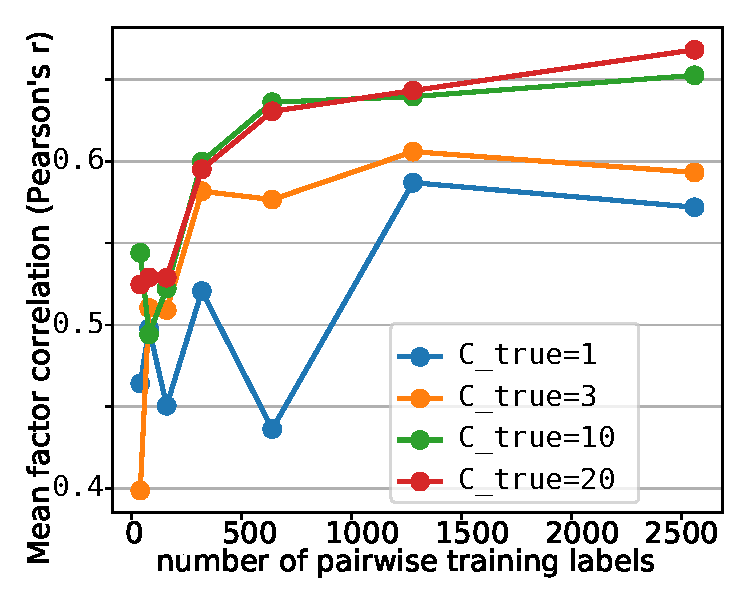
\includegraphics[width=.32\columnwidth,clip=true,trim=3 0 13 0]{../../results/synth_3/multi_factor_correlations_P/num_pairs_r}
}
\caption{Rank correlation between true and inferred preference values for different inference tasks.  (a) \& (b) varying level of noise in pairwise training labels, (d) varying number of pairwise training labels. 
}
\end{figure}
First, we test how well crowdGPPL is able to recover an underlying consensus function
from pairwise labels with varying amounts of noise.
We compare crowdGPPL against GPPL trained on all users' preference labels to learn a single  function (\emph{GPPL}), %and a Gaussian process over the joint feature space of users and items 
%(\emph{joint-GPPL}), as proposed by \citet{guo2010gaussian}.
%For datasets up to 100 users (simulated data, subsamples of the real datasets), 
and separate GPPL instances per user with no collaborative
learning (\emph{GPPL-per-user}). The consensus for GPPL-per-user is the mean of all users' predicted utilities. For all models, we set hyperparameters
$\alpha_0 = 2$, $\beta_0 = 2$ and, for crowdGPPL, $C=25$.

For the first test,
we generate data by selecting $100$ points at random
from a $10x10$ grid and choosing $500$ pairs of these points at random. 
We generate pairwise labels by drawing from crowdGPPL
with $25$ users, $5$ latent components, and 
$s=0.001$.
We vary the precision of the consensus function, $\sigma$ to control the noise in 
the consensus function. 
The chosen points are split into 50\% training and test sets.
%, and
%train our models on all pairs involving only points in the training set.
%We then predict the consensus function
% and personal utilities for all users 
%for the points in the test set.
%We repeat this process, varying the value of $s$ in the generation step, 
%which controls the precision of a latent preference function: as $s$ is increased, the latent
%function values have a smaller amplitude and the pairwise labels become noisier.
We repeat the complete experiment $25$ times, including generating new data 
for each value of $\sigma$.

%The results of the first test in Figure \ref{fig:simA} show that increasing
%the noise rate in the pairwise labels causes a near-linear decrease in the
%rank correlation between the predicted and true preference function values. 
%Nonetheless, GPPL is able to recover the ranking of points with $\tau > 0.5$ when
%more than $1/3$ pairwise labels are incorrect.
%we recover a consensus function
%from preference labels produced by multiple simulated users with varying differences
%in their individual preferences. We use the same process as the first simulation, except
%we now draw the pairwise labels from a crowdGPPL model  latent factors,
%instead of a single-user model. 
%We use three methods to recover the consensus function, GPPL-per-user, pooled-%GPPL, 
%and crowdGPPL with $C=25$ so that there is one factor per user. 
Figure \ref{fig:simB} shows that the crowdGPPL model is better able recover the latent consensus
function than the other methods, even when noise levels are high. 
The pooled model's predictions may be worsened by biased users whose preferences deviate
 consistently from the consensus. GPPL-per-user relies on separate instances of GPPL, so 
 does not benefit from sharing information between users when training the model.

The second simulation repeats the same setup as the first, 
but here we evaluate the methods'
ability to to recover the personal preferences of simulated users.
We fix $\sigma = 10$ and vary $s$.
Results in Figure \ref{fig:simC} show that crowdGPPL is able to make better 
predictions when noise is below $0.3$ but its benefit disappears when 
the noise level increases further. 

%In the final simulation, %we evaluate the effect of the quantity of training data 
%with different numbers of latent factors in the generating model.
We hypothesize that when the generating model has 
a larger number of latent components, more training data is required to learn
the more complex model.
%scenario that would require more training data. 
In the third simulation, we generate data using the same setup as before, but fix $s=0.2$ and $\sigma=1$
and vary the number of pairwise training labels 
and the number of true components through
$C_{true} \in \{ 1, 3, 10, 20\}$.
To evaluate the correlation between inferred and true user components, 
%we match inferred factors to true factors, 
we compute Pearson correlations between each
true component and each inferred component, then repeatedly select the pair of unmatched components with the highest correlation until all true components
are matched. 
In Figure \ref{fig:simD} we plot the mean of the correlations between matched pairs of components.
For all values of $C_{true}$, increasing the
number of training labels beyond $1000$ leads to only minor increases in correlation. Performance is best when $C_{true} = 20$,
possibly because the predictive model has $C = 25$
and hence is a closer match to the generating model.
However, performance with $>500$ labels remains above 0.5,
for all values of $C_{true}$, showing the model is reasonably robust
to mismatches between $C$ and $C_{true}$.
% Does this pose a question: does the mismatch affect the performance? If the correlations
% decrease, it may mean that the model is decomposing a factor into a sum of multiple factors,
% or it may just be unable to learn it. This would need a new experiment: for 700 training pairs,
% how does the accuracy of personalised predictions vary with the number of latent factors?
% I think this needs us to vary C and keep C_true=3, otherwise we don't know whether the 
% performance differences are due to the mismatched no. factors or due to different underlying dataset, i.e. we need to keep the data the same to compare!

\subsection{Argument Convincingness}\label{sec:exp_scale}

% TODO: split the personalised results by no. training examples per worker
% and by model confidence. Does filtering predictions with low confidence estimates
% help? Do workers with more data get better predictions?

We evaluate consensus learning, personal preference learning and scalability
on an NLP task, namely identifying convincing arguments. 
The dataset, \emph{UKPConvArgCrowdSample}, 
contains arguments written by users
of online debating forums
and crowdsourced judgments for pairs of arguments
 indicating the most convincing argument.
It is a subsample obtained by~\citet{simpson2018finding}
from the crowdsourced data provided by ~\citet{habernal2016argument}.
%The task is to quantify how convincing each argument is
%by learning a model from pairwise preference labels obtained from crowdworkers
%on Amazon Mechanical Turk. 
Each argument is are represented by $32,310$ numerical features and the
dataset is divided into $32$ folds ($16$ topics, each of which has two opposing stances). For each fold, we train on $31$ folds and test on the remaining fold.
%thereby performing a cross-topic evaluation.
%test the ability of the preference learning methods to predict the consensus
 %by training on raw crowdsourced pairwise labels
%for $31$ topics, and testing against the gold pairwise labels and rankings for the
%remaining topic. This process is repeated for all $32$ topics.
GPPL was previously shown to outperform SVM, Bi-LSTM and 
Gaussian process classifier methods at consensus prediction for \emph{UKPConvArgCrowdSample}~\citep{simpson2018finding}. 
%We compare GPPL with crowdGPPL and also test each method's 
%ability to predict the raw crowdsourced labels, i.e. the individual preference labels
%supplied by each worker.
We hypothesize that a worker's view of convincingness 
depends somewhat on their prior beliefs and understanding of the subject 
discussed and the language used, and therefore
%If this is the case, then provided that the data is sufficiently informative,
crowdGPPL may more accurately predict unseen 
pairwise labels or rankings for individual workers,
and may be better able to predict the consensus preference function by accounting 
for the biases of individual workers.

Table \ref{tab:convarg} shows performance for GPPL and crowdGPPL with the median
heuristic (\emph{medi.}) and with gradient-based optimization (\emph{opt.}).
CrowdGPPL outperforms GPPL at predicting the consensus pairwise labels
(all significant with $p<0.05$, Wilcoxon signed-rank test), 
shown by classification accuracy (\emph{acc}) and cross entropy error (\emph{CEE}),
and the consensus ranking ($p<0.05$), shown by Kendall's tau rank correlation (\emph{Kend}).
For the personal preference predictions, crowdGPPL outperforms 
GPPL at ranking ($p<0.05$) but pairwise label prediction performance is comparable.
This may be because the pairwise comparisons in the test folds are noisy and contain
numerous contradictions~\citep{habernal2016argument}, 
which are not present in the gold standard rankings, and hence are difficult to predict.
Length-scale optimization improves performance over the median heuristic,
although the difference is small and required approximately $5$ times longer to run.
% PERFORMANCE ----------------------------------------------------
% TODO: exclude tau from the personal column -- not enough data to compute the gold standard correctly, only pairwise labels are real gold!
% Things we could do:
% forget about trying to predict the crowd consensus, focus on scalability
% This means we don't need to show performance improvements against 
% Houlsby or for crowdGPPL for the consensus prediction.
% however, if we want to show that the optimization procedure has improved performance, we should find out why the consensus results for crowdGPPL are so bad. 
% It may be a data matchup error.
% Change to a different dataset instead of convincingness, or make sure to exclude workers with < 10 labels.
% For sushi, we can test on unseen users. This wasn't done by Khan or Houlsby. I guess
% that performance will be close to the pooled model, but it may help. This would
% demonstrate a benefit of the GP method.
\begin{table}
\begin{tabularx}{\columnwidth}{ | l | X | X | X | X | X | X |}
\hline
 & \multicolumn{3}{|X|}{Consensus}&\multicolumn{3}{| X |}{Personal} \\ \hline
 Method & Acc & CEE & Kend. & Acc & CEE & Kend. \\ \hline
 %SVM & .70 & .58 & .31 & .63 & .66 & .31 \\
 %Bi-LSTM & .73 &  .55 & .21 & .64 & .64 & .21 \\
 GPPL medi. & .77 & .50 & .40 & .71 & .56 & .32 \\
 GPPL opt. & .76 & .51 & .47 & .70 & .58 &  .30 \\
 crowdGPPL medi. & .78 & .48 & .51 & .71 & .59 & .32 \\
 crowdGPPL opt. & .78 & .48 & .50 & .69 & .59 & .29
 %PL+ SVR & .75 & .55 & \textbf{.40} & .75 & & .40 \\
 %GPC & .73 & .53 & - & .68 & .59 & - \\
 \\\hline
\end{tabularx}
\caption{Performance comparison on UKPConvArgCrowdSample using ling+GloVe features. \emph{Acc} and \emph{CEE} show classification accuracy and cross entropy error (or log-loss) for pairwise predictions, 
while \emph{Kend.} shows Kendall's tau for the predicted preference function.}
% wilcoxon signed-rank test: crowdGPPL vs. GPPL --> medi. p = 
\label{tab:convarg}
\end{table}
%TODO check why the results now show no difference between the methods --
% the performance appears to be more extreme, i.e. either much worse or much
% better with crowdGPPL. Folds where the transfer between domains works well -->
%crowdGPPL will work well. So how can we show this? Is the confidence higher
% on the better performing folds? Consider showing performance on more confident points only.
%TODO check whether evaluating accuracy on all pairs would be better than doing it
% per user -- currently the long tail of workers with few labels are getting too much
% weight. Problem would be if the workers with more labels on one fold have fewer
% on the training folds...

We assess our proposed SVI inference method by evaluating GPPL and crowdGPPL with
different numbers of inducing points, $M$. Figure \ref{fig:M} shows the trade-off between
runtime and accuracy as an effect of choosing $M$. Accuracy close to the peak is attained
using $M=200$, after which the accuracy levels off, while the runtime increases rapidly
as $M$ increases.
With $300$ features, the polynomial training time complexity is visible in the runtime. 
However, with $33,210$ features, the runtime plot appears almost linear, since 
the cost of computing covariance matrices, which is linear in the number of features,
dominates the runtimes. The plots show that the SVI method provides a substantial cut
in runtimes while maintaining good prediction accuracy.

Figures \ref{fig:Ntr} and \ref{fig:Npairs} show runtimes as a
function of the training set size, $N_{tr}$,
and the number of pairwise training labels, $P$, respectively.
The methods labeled "no SVI" show runtimes
for GPPL and crowdGPPL with variational inference but no stochastic updates 
or inducing points. 
When using SVI, runtimes increase very little 
with $N_{tr}$ or $P$. 
%These are compared with Bi-LSTM and SVM classifiers trained to 
%output probabilities of pairwise labels. 
%The plots clearly show the rapid increases
%in runtimes for these alternative methods. 
%For GPPL and crowdGPPL, 
%the cost of kernel computations becomes visible only with $33,210$ features, 
%indicating the benefits of more compact representations. BiLSTM appears unaffected by
%additional input dimensions, while the SVM runtimes increase noticably from $30$ to $300$ and $3000$ features.
% List of experiments to include -- need new plots for the crowd model:
% \begin{enumerate}
% \item Performance, computation time vs. no. inducing points
% \item Computation time vs. dataset size, no. features
% %\item not done: memory vs no. inducing points, update size
% %\item not done: Performance, computation time, vs update size
% %%\item not done: performance, computation time vs different initialisation methods for the inducing points; include different initialisations of K-means
% \end{enumerate}
% SCALABILITY ----------------------------------------------------------
\begin{figure}
\subfloat[300 GloVe features]{
 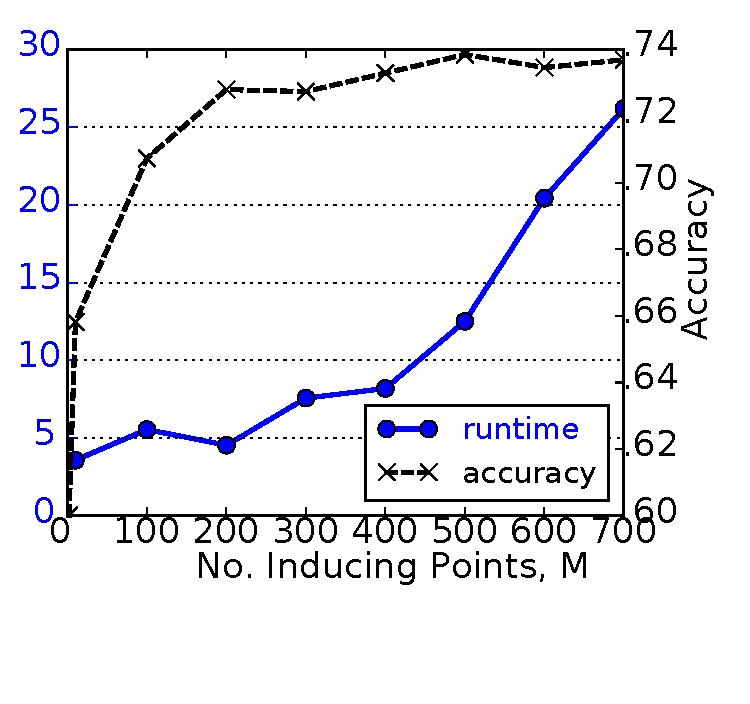
\includegraphics[width=.5\columnwidth]{../../results/scalability/num_inducing_300_features}
}
\subfloat[33210 ling+GloVe features]{
 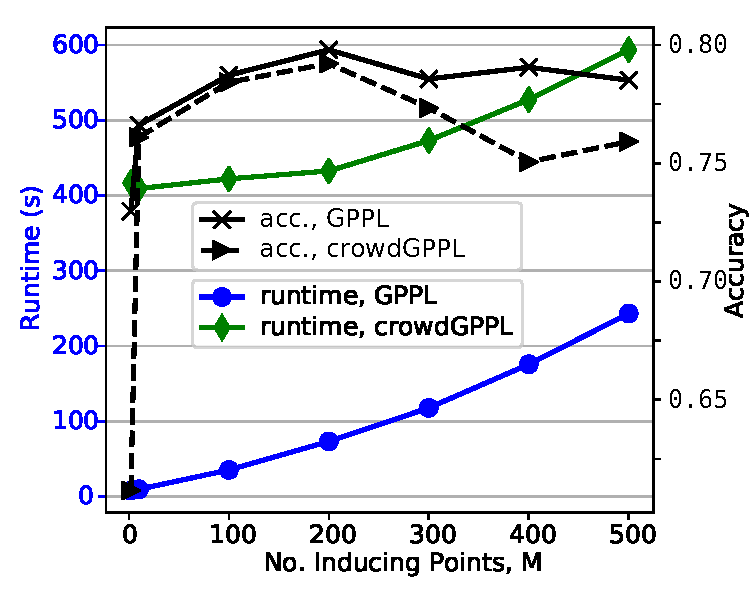
\includegraphics[width=.5\columnwidth]{../../results/scalability/num_inducing_32310_features}
}
\caption{
Effect of varying $M$ on accuracy and runtime (training+prediction) for GPPL and crowdGPPL on UKPConvArgCrowdSample. Means over 32 runs.
}
\label{fig:M}
\end{figure}
\begin{figure}
\subfloat[Varying number of items in training set.]{
\label{fig:Ntr}
%    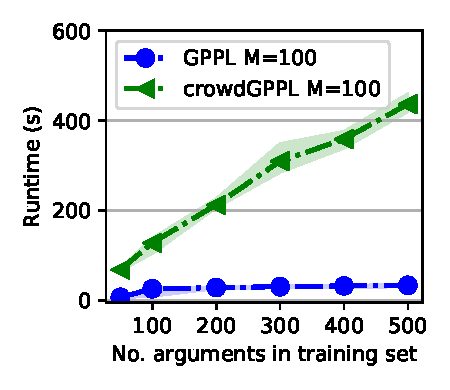
\includegraphics[width=.35\columnwidth]{../../results/scalability/num_arguments}
}
\subfloat[Varying no. pairwise training labels. ]{
\label{fig:Npairs}
 %   \includegraphics[width=.35\columnwidth]{../../results/scalability/num_features}
}
\caption{
    Runtimes for training+prediction on UKPConvArgCrowdSample with varying subsample size. 300 GloVe features. Means over 32 runs. 
    Note the logarithmic x-axis for (b).
}
\end{figure}

\subsection{Sushi Preferences}\label{sec:sushi}

%TODO sushi-A small needs describing or cutting out.
We use two datasets, Sushi-A and Sushi-B (shown in Table \ref{tab:datasets}),
to benchmark the classification and ranking performance of GPPL and crowdGPPL, 
as well as their runtimes, against previous approaches, 
and investigate the use of user features for predicting preferences.
The datasets contain, for each user, a gold standard preference ranking 
of $10$ types of sushi,
from which we generate gold-standard pairwise labels. 
%These labels can be considered noise-free, since
%they are derived directly from the gold standard ranking.  
For Sushi-A, we select a subset of $1000$ workers at random, then 
split the data into training and test sets by randomly
selecting $15$ pairs for each user for training and $5$ for testing. 
For Sushi-B, we use all $5000$ workers, and subsample $10$ training pairs and $1$ test pair per user.
Beside GPPL, crowdGPPL and GPPL-per-user, we 
% but this could not be applied to larger datasets as the 
%computation costs were too high.
introduce four further baselines: 
\emph{crowdGPPL$\mathbf{\setminus \bs u}$}, which ignores the user features;
 \emph{crowdGPPL$\mathbf{\setminus \bs u \setminus \bs x}$}, which ignores both user and item features and so does not use GPs at all;
 \emph{crowdGPPL$\mathbf{\setminus \bs u \setminus \bs t}$}, which 
excludes the consensus function $\bs t$ from the model as well as the user
features;
and  \emph{crowdGPPL$\backslash$induc}, which uses all features but does 
not use inducing points for a sparse approximation.
Standard crowdGPPL is labelled '\emph{full}'.
For these methods, the user covariance matrix, $\bs K_w$, in the crowdGPPL model is replaced by the identity matrix, and for crowdGPPL$\mathbf{\setminus \bs u \setminus \bs x}$, the item covariance matrices, $\bs K_v$ and $\bs K_t$ are also replaced by the identity matrix.
%We evaluate the quality of pairwise predictions using classification accuracy and cross entropy 
%error (also known as log loss) to gauge the quality of the probabilities that each method outputs.
%We also evaluate each method's inferred personal preference values
%against the gold standard rankings by computing Kendall's $\tau$ rank correlation
%coefficient between the negative rank and the inferred preference function values,
%for all the items contained in each subsampled user's ranking.
The complete process of subsampling, training and testing, was repeated $25$ times
for each dataset.

% Houlsby results: for comparison against a different inference technique on small data, include
% the test error results from their paper.
% Guo results: not directly comparable. We will rerun a similar approach but with our inference method.
% Khan results: for a different model that separates the latent features from the item/user features.
% Abbasnejad results (community-based preference learning): sushi data with 10 items; 60/40 train/test split of each user's preference pairs. This means the result is based on 27 pairs training.
% don't worry about this though, it doesn't seem to work very well in their results.

% Number of users affects value of including user features.
% Plot results on increasing dataset size.

% [10] T. Kamishima. Nantonac collaborative filtering:
% Recommendation based on order responses. In
% ACM SIGKDD 9th Int. Conf. Knowledge Discov-
% ery and Data Mining, 2003.

% Run 25 repeats of random train/test splits with:
% Exclude these two as we focus on bigger datasets in this paper. Cutting these creates the space 
% for including three metrics.
% Downside: cannot test whether increasing no. users imroves performance through better collaborative learning. 
% 
% 100 (a la Houlsby 20 pairs per user), 
% 200 (a la Khan, 3 training, 1 test, P=600, P_test=200), 
% For small datasets, we may want to test on the argumentation data so we can assess the crowd
% consensus results with small data. That dataset is more interesting here because lots of items,
% small data is a new scenario.
% % % % [a] 1000 (a la Houlsby 15 training, 5 test pairs per user, $P=15000,P_{test}=5000$), Sushi-A (10 items), 
% % % % and [b] 5000 users (a la Khan, 10 training, 1 test pairs per user, $P=50000, P_{test}=5000$), Sushi-B (100 items).
% % % % Evaluate on parwise labelling error, pairwise label logloss, spearman rank correlation,
% % % % and runtime.
% could use normalized mean loss from guo, but not sure where the utilities come from -- ranking?

% 25 random train/test splits on all 5000 users with varying no. (1, 5, 10, 20, 40) pairs per user.

% Can put in the Houlsby (100/1000 users, 20 pairs each, labelling error) and Khan (200 users, 3 pairs each, logloss) results.
% Khan also provide code, so could be rerun to get classification error.

\begin{table}
\small
\begin{tabularx}{\textwidth}{| p{1.1cm} | X | X | X | p{0.55cm} | X | X | X | p{0.7cm} | X | X | X | p{0.7cm} |}
\hline
& \multicolumn{4}{c|}{\textbf{Sushi-A-small}} & \multicolumn{4}{c|}{\textbf{Sushi-A}} & \multicolumn{4}{c|}{\textbf{Sushi-B}} \\ 
Method & Acc & CE E & $\tau$ & Run-time & Acc & CE E & $\tau$ & Run-time & Acc & CE E & $\tau$ & Run-time \\
\hline\hline
\multicolumn{13}{|l|}{\textit{crowdGPPL}} \\
full & .67 & .87 & .39 & 77%76.91 %(27.23) %& .63 (.02) & .69 (.00) & .25 (.02)
& .79 & .51 & .66 & 150%149.6 %(20.86)
& .69 & 2.23 & .45 & 9163 
\\
full, opt. & & & & & .80 & .48 & .68 & 3718 
& - & - & - & - 
\\%(2193.72) \\
$\backslash $induc & .70 & \textbf{.57} & .46 & 166 %(14.81) %& .63 (.02) & .68 (.00) & .24 (.03)
& .84 & \textbf{.33} & .79 & 315 %(50.17) 
& - & - & - & -
\\
%$\backslash t$ & .67 & .80 & .39 & 7.45 (29.00) %& .61 (.02) & .69 (.00) & .19 (.03)
%& .79 & .57 & .65 & 158.51 (25.06)
%\\
$\backslash u$ & .70 & .58 & .46 & 175 %(24.62) %& .65 (.02) & .64 (.03) & .29 (.03)
& .84 & \textbf{.33} & \textbf{.80} & 336 %(4.93)
& \textbf{.76} & \textbf{.47} & \textbf{.60} & 21052
\\
$\backslash u$, opt. & & & & & \textbf{.85} & \textbf{.33} &  \textbf{.80} & 5016 %(1978.82) \\
& - & - & - & - \\
$\backslash u \backslash x$ & \textbf{.71} & \textbf{.57} & \textbf{.49} & 5 %(3.74) %& .65 (.02) & .63 (.02) & .29 (.03)
& \textbf{.85} & \textbf{.33} & \textbf{.80} & 329 %(12.12)
& \textbf{.76} & .48 & \textbf{.60} & 15478
\\
%$\backslash u$, FITC & .70 & .58 & .46 & 333.68 (57.36) %& .65 (.01) & .64 (.02) & .29 (.02)
%& \textbf{.85} & \textbf{.33} & \textbf{.80} & 551.56 (16.82)
%\\
$\backslash u$$\backslash t$ % this is also FITC to emulate Houlsby -- mention it in the text, not here
& .68 & .60 & .43 & 291 %(48.62) %& .50 (.00) & .69 (.00) & nan (nan)
& .84 & \textbf{.33} & .79 & 540 %(12.15) 
& .75 & .49 & .59 & 30484
\\ 
%$\backslash u$$\backslash t$, FITC, opt. & & & &  & .84 & \textbf{.33} & \textbf{.80} & 7413.53 (2849.63) \\
\hline 
GPPL & .65 & .62 & .31 & \textbf{2} %(.26) %& .65 (.02) & .63 (.02) & .30 (.03)
& .66 & .62 & .32 & \textbf{2} %(.38) & 
& .65 & .62 & .31 & \textbf{51}
\\
GPPL-per-user & .67 & .64 & .42 & 97 %(1.12) %& .50 (.00) & .69 (.00) & nan (nan)
& .83 & .40 & .79 & 67 & .75 & .60 & \textbf{.60} & 18078 %(.44)
\\
\hline
%\citet{houlsby2012collaborative} CP & & & & & .84 \\
%\citet{houlsby2012collaborative} CPU & & & & & .83 \\ 
%\citet{khan2014scalable} & &&& & & & & & .69 & &
%\\ \hline
\end{tabularx}
\caption{Predicting personal preferences: performance on Sushi-A dataset and Sushi-B datasets.
Runtimes given in seconds, with standard deviation between repeats in brackets.
For accuracy, all standard deviations are $\leq 0.02$, for CEE $\leq 0.08$, for Kend. $\leq 0.03$.
 }
\label{tab:sushi}
\end{table}
%  -- the stds were removed because they're not very informative for acc, CEE, tau
% The commented results are predictions on new users -- for sushiAsmall, the only interesting 
% point is that excluding the consensus decreases accuracy. How does it make predictions without a t?
The results in Table \ref{tab:sushi} 
%we re-state the previous performance metrics and did not re-implement these methods. 
illustrate the benefit of crowd models over single-user GPPL.
The runtimes 
show that including feature data for items and users leads to faster convergence than crowdGPPL$\backslash \bs u$ and crowd$\backslash \bs u \backslash \bs x$.
%Likewise, the use of matrix factorization leads to only a small increase in
% runtimes of these methods over joint-GPPL. 
 However, the runtimes for crowdGPPL are higher than those of GPPL.
 When using inducing points, the user features decrease the performance of crowdGPPL: the methods \emph{crowdGPPL$\backslash$induc}
 and \emph{crowdGPPL$\backslash\bs u$} both outperform the full crowdGPPL. 
 When using inducing points,
 there must be a strong relationship between neighbouring points, which
 is likely not to be the case given the features in this dataset.
 Again, we see small improvements in performance after length-scale optimization,
 but this takes approximately 22 times as long to train.
% as are the performance metrics. 
CrowdGPPL produces similar classification scores to the earlier method of 
 \citep{houlsby2012collaborative} (0.83 on Sushi-A with user features, and 0.84 without), 
 while using a more scalable inference method.
Performance is also improved over that of \citep{khan2014scalable}, which 
attained CEE=0.69 n Sushi-B using
 a GP for each user in combination with Bayesian matrix factorization. 
GPPL-per-user performs well on Sushi-A, but does not perform as well as other methods on Sushi-B.
%Figure \ref{fig:latent_factor_variance} again shows that the inferred crowdGPPL model relies
%heavily on a subset of the latent factors.
% We should bring the scalability experiments forward so that we don't need the runtimes here?
% Or so we can at least avoid comparing with Houlsby and Khan on runtimes. 
% The Khan runtime should be GPPL-per-user + BMF. However, the interconnection of the two might 
% make them take more or less time?

\subsection{Posterior Variance of Item Components}
\label{sec:components}

We investigate how many latent components were actively used by 
 crowdGPPL on the UKPConvArgCrowdSample and Sushi-A datasets 
 using the median heuristic.
Figure \ref{fig:latent_factor_variance}
plots the posterior expectations of the inferred scales, $1/s_c$, for the latent item 
 components. 
 The plots show
that many factors have a very small variance and therefore do not contribute strongly 
to the model's predictions. This indicates that our Bayesian approach, in which the priors
of the latent factors have mean zero, has inferred a simpler model even when
 a larger number of latent components was available.
\begin{figure}
\centering
\subfloat[UKPConvArgCrowdSample]{
\includegraphics[trim=10 0 3 0,clip=true,width=.4\textwidth]{../../results/conv_factors/UKPConvArgCrowdSample_factor_scales.pdf}
}
\subfloat[Sushi-A]{
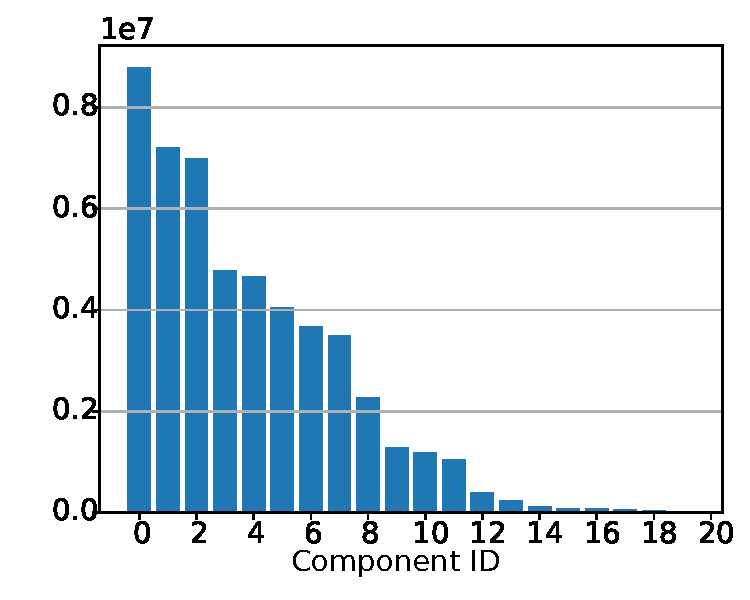
\includegraphics[trim=20 0 0 0,clip=true,width=.4\textwidth]{../../results/sushi_factors/sushi_factor_scales}
}
\caption{
Distribution of latent factor variances, $1/s_c$, for crowdGPPL on UKPConvArgCrowdSample, Sushi-A and Sushi-B, averaged over all runs.
}
\label{fig:latent_factor_variance}
\end{figure}
\section{Conclusions}

We proposed a Bayesian preference learning approach 
for modeling both the individual utilities of members of a crowd 
and forming a consensus from 
unreliable annotations, such as those provided by a crowd or through implicit user feedback.
The model learns the latent utilities of items from pairwise comparisons using a combination of Gaussian processes and Bayesian matrix factorization.
To enable inference at the scale of real-world datasets in fields such as NLP,
we derived a stochastic variational inference scheme.
Our empirical results confirm that our approach scales far better than previous
Gaussian process preference learning methods without harming  
performance on individual utility prediction and significantly improving performance
on consensus learning.
Future work will evaluate the benefit of learning inducing point locations from data,
and investigate the possibility of integrating deep generative models 
for learning feature representations from input data.
%the models can readily be adapted to regression or classification tasks by swapping out the preference likelihood, resulting in 
%different values for $\bs G$ and $\bs H$.


%%%%%%%%%%%%%%%%%%%%%%%%%%%%%%%%%%%%%%%%%%%%%%%%%%%%%%%%%%%%%%%%%%%%%%%%%%%%%%%%

% use section* for acknowledgment
\section*{Acknowledgments}

\cleardoublepage

\bibliographystyle{spbasic}
\bibliography{simpson_scalable_bayesian_pref_learning_from_crowds}

%%%%%%%%%%%%%%%%%%%%%%%%%%%%%%%%%%%%%%%%%%%%%%%%%%%%%%%%%%%%%%%%%%%%%%%%%%%%%%%%%

\end{document}
